\newif\ifglobal

%%%%%%%%%%%%%%%%%%%%%%%
%%% Compile to view %%%
%%%%%%%%%%%%%%%%%%%%%%%

%%%%%%%%%%%%%%%%%%%%%%%%%%%%%%%%%%%%%%%%%%%%%%%%%%%
%%% Readme:                                     %%%
%%% https://www.overleaf.com/read/bwdjvfjksvjy/ %%%
%%%%%%%%%%%%%%%%%%%%%%%%%%%%%%%%%%%%%%%%%%%%%%%%%%%

% >>> M?: marks a module setting number or important notice

% >>> M4: Set {./relative-path} to external files for this module <<<
\def \modulefiles {./01-I2C}
% To add an external file, use:
% (Replace '---' with actual filename)
% '\input{\modulefiles/tables/---.tex}' for tables
% '\includegraphics{\modulefiles/figures/---}' for figures
% '\subfile{\modulefiles/---}' for register files

% >>> M1: This module is in global project? <<<
% 'YES' - uncomment; 'NO' - comment out
\globaltrue

\ifglobal
    \documentclass[main\_\_CN.tex]{subfiles}

\else
    % Font "FandolSong-Regular" used by ctex does not have GSUB table.
    % It causes warnings that do not affect compilation and can be ignored.
    \PassOptionsToPackage{quiet}{fontspec}

    \documentclass[openany, 10pt]{book}

    % >>> M2: In ./00-shared/preamble-trm-module, also find
    %         settings for visibility of todo notes, watermark <<<
    \usepackage{preamble-trm-module}


    % Enable Chinese typesetting
    \usepackage{ctex}

    % >>> M3: Temporary labels in Chinese
    %         you can add your own labels there <<<
    \myexternaldocument{./00-shared/temp-labels-cn}

\fi %\ifglobal


\setcounter{secnumdepth}{4}

% >>> M4: Set {./relative-path} to external files for this module <<<
% \def \modulefiles {./01-I2C}
% To add an external file, use:
% (Replace '---' with actual filename)
% '\input{\modulefiles/tables/---.tex}' for tables
% '\includegraphics{\modulefiles/figures/---}' for figures
% '\subfile{\modulefiles/---}' for register files


% >>> M5: If this module needs any updates in
% './00-shared/preamble-trm-module.sty'
% (include additional package, etc.), contact your module PM
% or create the file './00-shared/changelog.tex' make the
% necessary updates yourself and document them in this file <<<


\begin{document}


% Sets language into which pre-defined bits of text are translated
\selectlanguage{chinese}

% Do not delete this block
\ifglobal
% Add the following front matter if
% this module is outside of global project
\else
    \InputIfFileExists{readme}{}{}
    {\let\clearpage\relax \listoftodos}
    \tableofcontents
    %\listoftables
    %\listoffigures
\fi


%%%%%%%%%%%%%%%%%%%%%%%%%
%%% TRM Module Begins %%%
%%%%%%%%%%%%%%%%%%%%%%%%%

\hypertarget{i2c}{}
\chapter{I2C 控制器 (I2C)}
\label{mod:i2c}



I2C (Inter-Integrated Circuit) 总线用于使 \chipname{} 和多个外部设备进行通信。多个外部设备可以共用一个 I2C 总线。


\section{概述}
I2C 是一个两线总线,由 SDA 线和 SCL 线构成。这些线设置为漏极开漏 (open-drain) 输出。因此,I2C 总线上可以挂载多个外设,通常是和一个或多个主机以及一个或多个从机。但同一时刻只有一个主机能占用总线访问一个从机。

主机发出开始信号,则通讯开始:在 SCL 为高电平时拉低 SDA 线,主机将通过 SCL 线发出 9 个时钟脉冲。前 8 个脉冲用于传输 7 位地址和 1 个读写位。如果从机地址与该 7 位地址一致,那么从机可以通过在第 9 个脉冲拉低 SDA 线来应答。接下来,根据读/写标志位,主机和从机之间可以传输更多的数据。根据应答位的逻辑电平决定是否停止发送数据。在数据传输中,SDA 线仅在 SCL 线为低电平时才发生变化。当主机完成通讯,发送一个停止标志:在 SCL 为高电平时,拉高 SDA 线。如果一次通信中主机既有写操作又有读操作,则主机需在读写操作变化前,发送一个重新开始信号、从机地址和读写标志位。重新开始信号不仅用于一次通信中切换方向,也用于切换设备模式(主机或从机模式)。

\section{主要特性}

I2C具有以下几个特点:

\begin{itemize}
    \item 支持主机模式和从机模式
    \item 支持多主机和从机通信
    \item 支持标准模式 (100 Kbit/s)
    \item 支持快速模式 (400 Kbit/s)
    \item 支持 7 位以及 10 位地址寻址
    \item 支持拉低 SCL 时钟实现连续数据传输
    \item 支持可编程数字噪声滤波功能
    \item 支持从机地址和从机内存或寄存器地址的双寻址模式
\end{itemize}

\section{I2C 架构}
\begin{figure}[H]
    \centering
    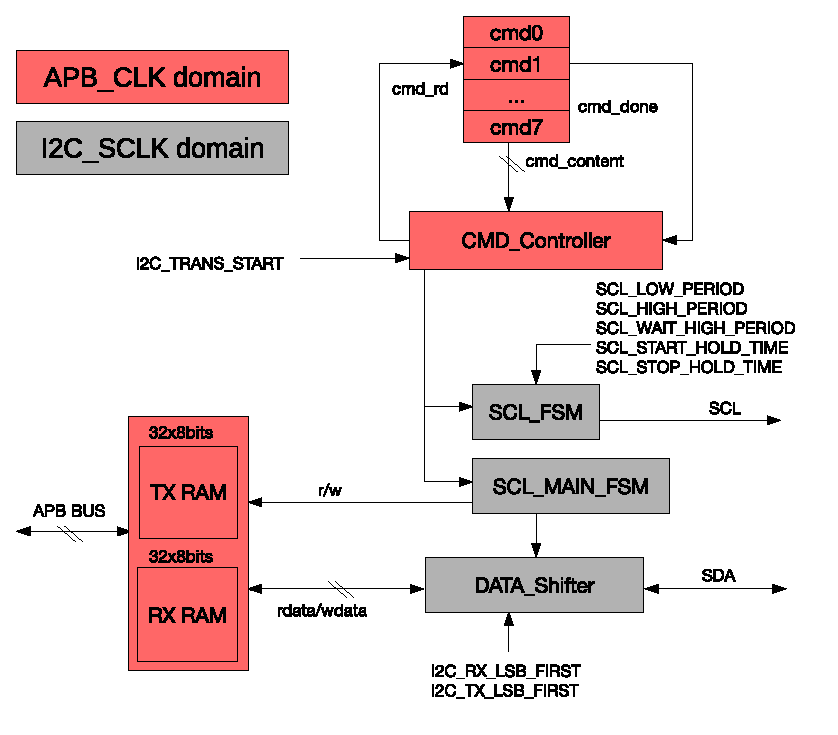
\includegraphics[width=0.65\textwidth]{\modulefiles/figures/728_i2c_master_architecture}
    \caption{I2C 主机基本架构}
    \label{fig:i2c-master}
\end{figure}

\begin{figure}[H]
    \centering
    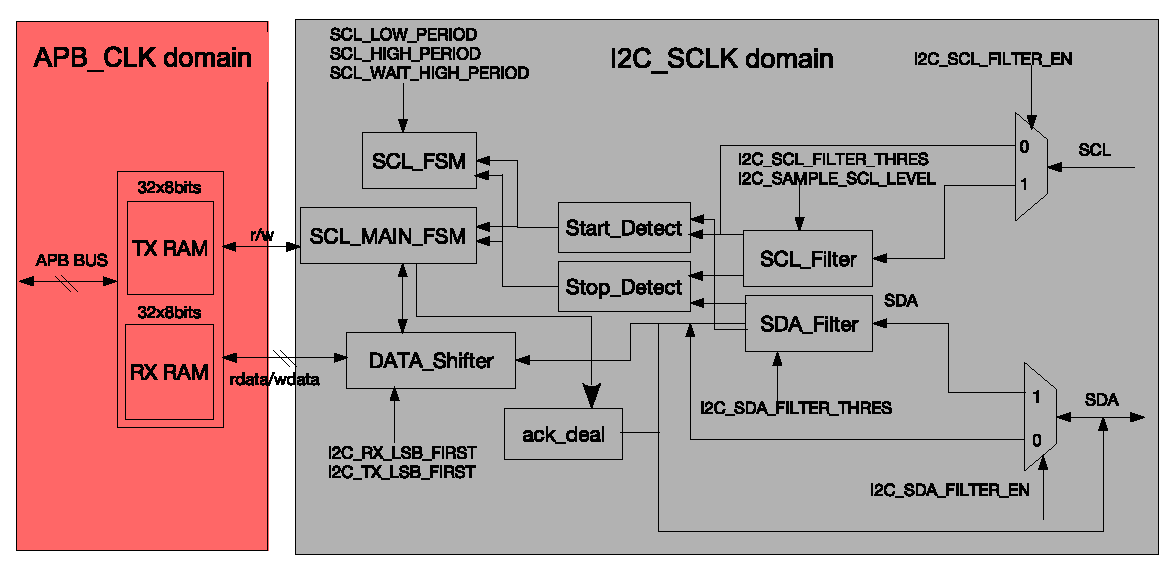
\includegraphics[width=0.8\textwidth]{\modulefiles/figures/728_i2c_slave_architecture}
    \caption{I2C 从机基本架构}
    \label{fig:i2c-slave}
\end{figure}

I2C 控制器可以工作于主机模式或者 从机模式,\hyperref[fielddesc:I2CMSMODE]{I2C\_MS\_MODE} 寄存器用于模式选择。图 \ref{fig:i2c-master} 为 I2C 主机基本架构图,图 \ref{fig:i2c-slave} 为 I2C 从机基本架构图。I2C 控制器内部包括的模块主要有:
\begin{itemize}
    \item 接收和发送存储器 TX/RX RAM
    \item 命令控制器 CMD\_Controller
    \item SCL 时钟控制器 SCL\_FSM
    \item SDA 数据控制器 SCL\_MAIN\_FSM
    \item 串并转换器 DATA\_Shifter
    \item SCL 滤波器 SCL\_Filter
    \item SDA 滤波器 SDA\_Filter
\end{itemize}

另外,还有产生 I2C 内部时钟的时钟模块,以及在 APB 总线和 I2C 模块之间同步的同步模块。

时钟模块的作用是进行时钟源选择,时钟开关和时钟分频。SCL\_Filter 和 SDA\_Filter 分别用于消除 SCL 及 SDA 输入信号上的噪声。同步模块用来同步不同时钟域之间信号的传输。

图 \ref{fig:i2c-protocol-timing} 和图 \ref{fig:i2c-timing-param} 是I2C协议的时序图和对应的参数表。SCL\_FSM 用来产生满足 I2C 协议的 SCL 时钟。

SCL\_MAIN\_FSM 模块用来控制 I2C 指令的执行,和 SDA线的序列。I2C 主机通过 CMD\_Controller 产生( R)START、STOP、WRITE、READ 和 END 指令。TX/RX RAM 分别用来存储 I2C 要发送和接收到的数据。DATA\_Shifter 用来完成串行数据和并行数据之间的转换。

\begin{figure}[H]
    \centering
    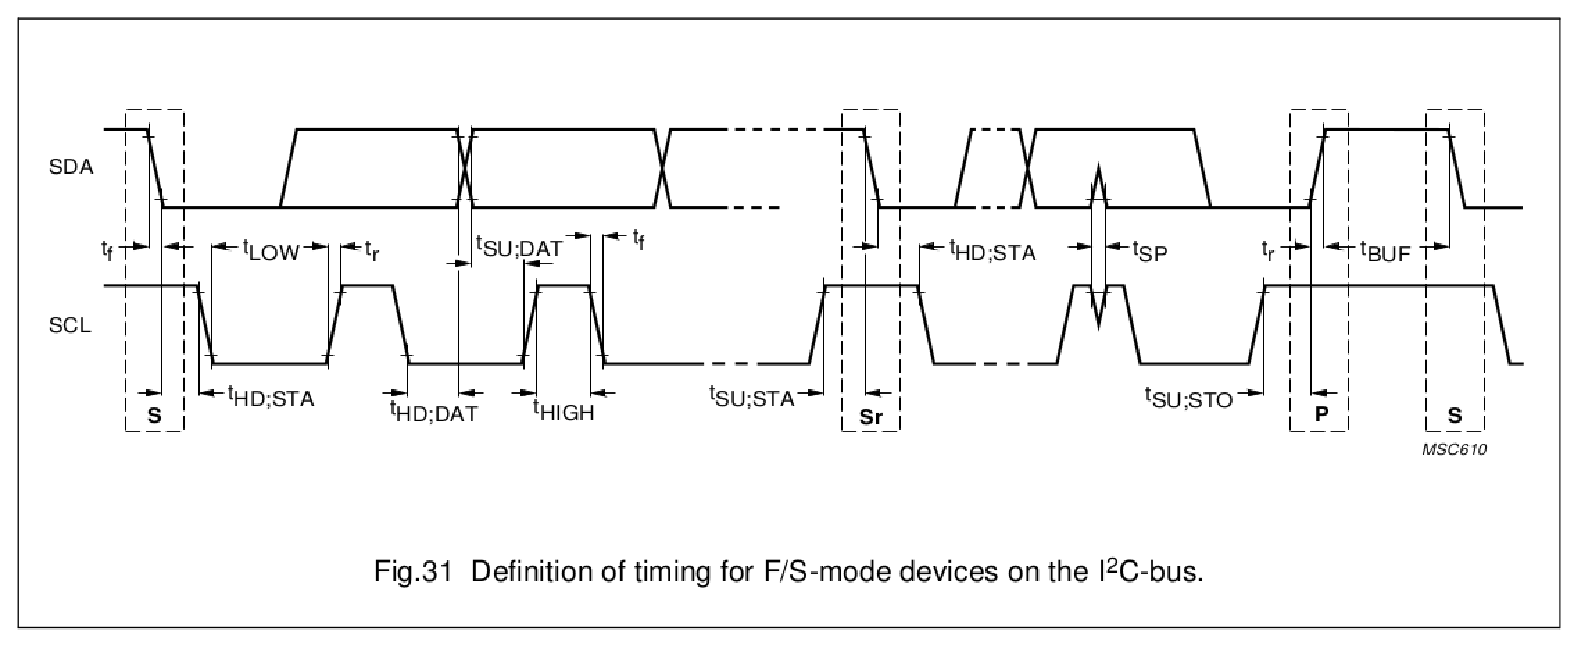
\includegraphics[width=0.9\textwidth]{\modulefiles/figures/i2c_timing_definition}
    \caption{I2C 协议时序(引自 \href{https://www.csd.uoc.gr/~hy428/reading/i2c_spec.pdf}{The I2C-bus specification} Version 2.1 Fig.31)}
    \label{fig:i2c-protocol-timing}
\end{figure}

\begin{figure}[H]
    \centering
    \fbox{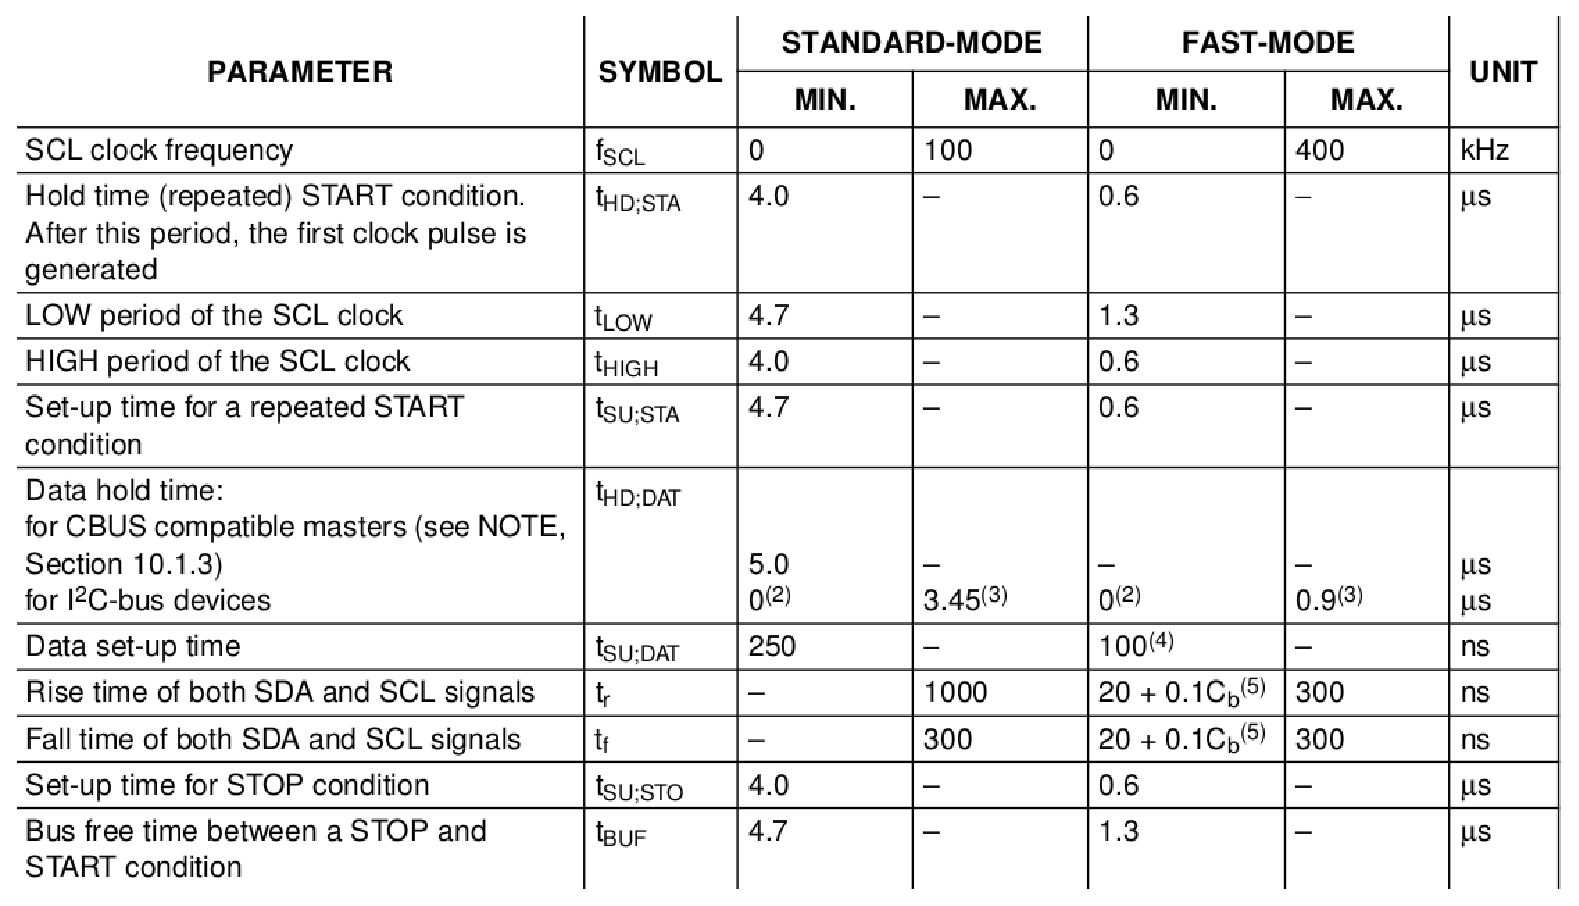
\includegraphics[width=0.9\textwidth]{\modulefiles/figures/i2c_timing_characteristic}}
    \caption{I2C 时序参数(引自 \href{https://www.csd.uoc.gr/~hy428/reading/i2c_spec.pdf}{The I2C-bus specification} Version 2.1 Table5)}
    \label{fig:i2c-timing-param}
\end{figure}

\clearpage
\section{功能描述}
需要注意的是,I2C 总线上其他主机或者从机的操作可能与 \chipname{} I2C 外设有所不同,具体请参考各个 I2C 设备的技术规格书。

\subsection{时钟配置}
寄存器配置和 TX/RX RAM 部分的时钟域为 APB\_CLK,时钟范围是 1 $\sim$ 80 MHz。I2C 主要逻辑部分,包括 SCL\_FSM、SCL\_MAIN\_FSM、SCL\_FILTER、SDA\_FILTER 和 DATA\_SHIFTER 都为 I2C\_SCLK 时钟域。

用户可以通过配置 \hyperref[fielddesc:I2CSCLKSEL]{I2C\_SCLK\_SEL} 选择 I2C\_SCLK 的时钟源:XTAL\_CLK 或 RC\_FAST\_CLK,\hyperref[fielddesc:I2CSCLKSEL]{I2C\_SCLK\_SEL} 为 0 时选择时钟源 XTAL\_CLK,\hyperref[fielddesc:I2CSCLKSEL]{I2C\_SCLK\_SEL} 为 1  时选择时钟源 RC\_FAST\_CLK。配置 \hyperref[fielddesc:I2CSCLKACTIVE]{I2C\_SCLK\_ACTIVE} 为高电平来打开 I2C\_SCLK 的时钟源。选择后的时钟经过小数分频得到I2C的工作时钟 I2C\_SCLK,分频系数为:
\[
I2C\_SCLK\_DIV\_ NUM + 1+\frac{ \hyperref[fielddesc:I2CSCLKDIVA]{I2C\_SCLK\_DIV\_A}}{\hyperref[fielddesc:I2CSCLKDIVB]{I2C\_SCLK\_DIV\_B}}
\]

XTAL\_CLK 的频率是 40 MHz,RC\_FAST\_CLK 的频率是 17.5 MHz。根据时序参数的限制,分频后的 I2C\_SCLK 的频率要满足大于 SCL 频率的 20 倍的关系。

\subsection{滤除SCL和SDA噪声}
SCL\_Filter 和 SDA\_Filter 滤波器模块实现方式相同,用于滤除 SCL 及 SDA 输入信号上的噪声。通过配置\\\hyperref[fielddesc:I2CSCLFILTEREN]{I2C\_SCL\_FILTER\_EN} 以及 \hyperref[fielddesc:I2CSDAFILTEREN]{I2C\_SDA\_FILTER\_EN} 寄存器可以开启或关闭滤波器。

以 SCL\_Filter 为例,当使能SCL\_Filter 功能时,滤波器会连续采样输入信号 SCL,如果输入信号在连续 \\\hyperref[fielddesc:I2CSCLFILTERTHRES]{I2C\_SCL\_FILTER\_THRES} 个 I2C\_SCLK 时钟周期内保持不变,则输入信号有效,否则输入信号无效。只有有效的输入信号才能通过滤波器。因此,SCL\_Filter 和 SDA\_Filter 滤波器会
过滤脉冲宽度小于 \hyperref[fielddesc:I2CSCLFILTERTHRES]{I2C\_SCL\_FILTER\_THRES} 以及 \hyperref[fielddesc:I2CSDAFILTERTHRES]{I2C\_SDA\_FILTER\_THRES} 个 I2C\_SCLK 时钟周期的线路毛刺。

\subsection{SCL 时钟拉伸}
从机模式下,可以通过拉低 SCL 线,给软件足够的时间处理数据。置位 \hyperref[fielddesc:I2CSLAVESCLSTRETCHEN]{I2C\_SLAVE\_SCL\_STRETCH\_EN} 位使能 SCL 时钟拉伸功能,配置 \hyperref[fielddesc:I2CSTRETCHPROTECTNUM]{I2C\_STRETCH\_PROTECT\_NUM} 字段来控制 SCL 拉伸后释放的时长以防出现时序错误。出现以下四种情况时从机会拉低 SCL 线:

\begin{enumerate}
\item 地址命中:从机模式下,从机地址与主机发送到 SDA 线上的地址相匹配,且读写标志位为 1。
\item 写满:从机模式下,I2C 控制器的 RX RAM 为满。注意,从机在接收少于 32 个字节时,可以不开启时钟拉伸功能;当要接收不少于 32 个字节时,可以通过 FIFO 阈值中断写 RAM 的乒乓操作,或者开始时钟拉伸功能,给软件提供处理时间。开启时钟拉伸功能时,必须将 \hyperref[fielddesc:I2CRXFULLACKLEVEL]{I2C\_RX\_FULL\_ACK\_LEVEL} 置 0,来保证功能正确,否则可能会出现不可预计的后果。
\item 读空:从机模式下,I2C 控制器要发送数据,但TX RAM 为空。
\item 发送 ACK 时:从机模式下置位 \hyperref[fielddesc:I2CSLAVEBYTEACKCTLEN]{I2C\_SLAVE\_BYTE\_ACK\_CTL\_EN},从机会在发送 ACK 时拉低 SCL。软件在此阶段进行一些操作,如数据校验,并通过配置\hyperref[fielddesc:I2CSLAVEBYTEACKLVL]{I2C\_SLAVE\_BYTE\_ACK\_LVL}控制将要发送的 ACK 的电平高低。要注意的是,当出现从机接收的 RX RAM 满时,要发送的 ACK 电平将由 \hyperref[fielddesc:I2CRXFULLACKLEVEL]{I2C\_RX\_FULL\_ACK\_LEVEL} 而不是 \hyperref[fielddesc:I2CSLAVEBYTEACKLVL]{I2C\_SLAVE\_BYTE\_ACK\_LVL} 决定。此时同样需要将 \hyperref[fielddesc:I2CRXFULLACKLEVEL]{I2C\_RX\_FULL\_ACK\_LEVEL} 置 0,以保证SCL 时钟拉伸功能的正常产生。
\end{enumerate}

SCL 线拉低后,软件可读取 \hyperref[fielddesc:I2CSTRETCHCAUSE]{I2C\_STRETCH\_CAUSE} 位获取SCL 时钟拉伸的原因。置位 \hyperref[fielddesc:I2CSLAVESCLSTRETCHCLR]{I2C\_SLAVE\_SCL\_STRETCH\_CLR} 位关闭 SCL时钟拉伸。

\subsection{SCL 空闲时产生 SCL 脉冲}
通常情况下,在 I2C 总线空闲时,SCL 线一直为高。\chipname{} I2C 支持在 I2C 主机处于空闲状态时,可编程配置产生 SCL 脉冲的功能。这个功能仅在I2C控制器作为主机时有效。置位 \hyperref[fielddesc:I2CSCLRSTSLVEN]{I2C\_SCL\_RST\_SLV\_EN},硬件会发送 \hyperref[fielddesc:I2CSCLRSTSLVNUM]{I2C\_SCL\_RST\_SLV\_NUM} 个 SCL 脉冲。一段时间后,软件读取到 \hyperref[fielddesc:I2CSCLRSTSLVEN]{I2C\_SCL\_RST\_SLV\_EN} 位的值为0后,再置位 \hyperref[fielddesc:I2CCONFUPGATE]{I2C\_CONF\_UPGATE},来停止这个功能。

\subsection{同步}
I2C 的寄存器配置用 APB 时钟,I2C 主模块用 I2C\_SCLK,这之间存在异步处理,需要增加同步的步骤将配置寄存器的值更新进入 I2C 主模块。步骤为先写配置寄存器,再向 \hyperref[fielddesc:I2CCONFUPGATE]{I2C\_CONF\_UPGATE} 位写 1。需要通过这种方法更新的配置寄存器详见表 \ref{tab:i2c-sync-register}。

\begin{longtable}{ | p{6cm} | p{7cm} | p{2cm} | }
\caption{I2C 同步寄存器}\label{tab:i2c-sync-register}\\\hline
\rowcolor{lightgray}
配置寄存器& 配置参数 & 地址  \\ \hline
\hyperref[regdesc:I2CCTRREG]{I2C\_CTR\_REG} & {\hyperref[fielddesc:I2CSLVTXAUTOSTARTEN]{I2C\_SLV\_TX\_AUTO\_START\_EN}} & 0x{}0004  \\\cline{2-2}

& {\hyperref[fielddesc:I2CADDR10BITRWCHECKEN]{I2C\_ADDR\_10BIT\_RW\_CHECK\_EN}}& \\\cline{2-2}
& {\hyperref[fielddesc:I2CADDRBROADCASTINGEN]{I2C\_ADDR\_BROADCASTING\_EN}}& \\\cline{2-2}
& {\hyperref[fielddesc:I2CSDAFORCEOUT]{I2C\_SDA\_FORCE\_OUT}}& \\\cline{2-2}
& {\hyperref[fielddesc:I2CSCLFORCEOUT]{I2C\_SCL\_FORCE\_OUT}}& \\\cline{2-2}
& {\hyperref[fielddesc:I2CSAMPLESCLLEVEL]{I2C\_SAMPLE\_SCL\_LEVEL}}& \\\cline{2-2}
& {\hyperref[fielddesc:I2CRXFULLACKLEVEL]{I2C\_RX\_FULL\_ACK\_LEVEL}}& \\\cline{2-2}
& {\hyperref[fielddesc:I2CMSMODE]{I2C\_MS\_MODE}}& \\\cline{2-2}
& {\hyperref[fielddesc:I2CTXLSBFIRST]{I2C\_TX\_LSB\_FIRST}}& \\\cline{2-2}
& {\hyperref[fielddesc:I2CRXLSBFIRST]{I2C\_RX\_LSB\_FIRST}}& \\\cline{2-2}
& {\hyperref[fielddesc:I2CARBITRATIONEN]{I2C\_ARBITRATION\_EN}}& \\ \hline

\hyperref[regdesc:I2CTOREG]{I2C\_TO\_REG} & {\hyperref[fielddesc:I2CTIMEOUTEN]{I2C\_TIME\_OUT\_EN}} & 0x{}000C  \\\cline{2-2}
& {\hyperref[fielddesc:I2CTIMEOUTVALUE]{I2C\_TIME\_OUT\_VALUE}}& \\ \hline

\hyperref[regdesc:I2CSLAVEADDRREG]{I2C\_SLAVE\_ADDR\_REG} & {\hyperref[fielddesc:I2CADDR10BITEN]{I2C\_ADDR\_10BIT\_EN}} & 0x{}0010 \\\cline{2-2}
& {\hyperref[fielddesc:I2CSLAVEADDR]{I2C\_SLAVE\_ADDR}}& \\ \hline


\hyperref[regdesc:I2CFIFOCONFREG]{I2C\_FIFO\_CONF\_REG} & {\hyperref[fielddesc:I2CFIFOADDRCFGEN]{I2C\_FIFO\_ADDR\_CFG\_EN}} & 0x{}0018 \\ \hline

\hyperref[regdesc:I2CSCLSPCONFREG]{I2C\_SCL\_SP\_CONF\_REG} & {\hyperref[fielddesc:I2CSDAPDEN]{I2C\_SDA\_PD\_EN}} & 0x{}0080  \\\cline{2-2}
& {\hyperref[fielddesc:I2CSCLPDEN]{I2C\_SCL\_PD\_EN}}& \\\cline{2-2}
& {\hyperref[fielddesc:I2CSCLRSTSLVNUM]{I2C\_SCL\_RST\_SLV\_NUM}}& \\\cline{2-2}
& {\hyperref[fielddesc:I2CSCLRSTSLVEN]{I2C\_SCL\_RST\_SLV\_EN}}& \\ \hline


\hyperref[regdesc:I2CSCLSTRETCHCONFREG]{I2C\_SCL\_STRETCH\_CONF\_REG} & {\hyperref[fielddesc:I2CSLAVEBYTEACKCTLEN]{I2C\_SLAVE\_BYTE\_ACK\_CTL\_EN}} & 0x{}0084  \\\cline{2-2}
& {\hyperref[fielddesc:I2CSLAVEBYTEACKLVL]{I2C\_SLAVE\_BYTE\_ACK\_LVL}}& \\\cline{2-2}
& {\hyperref[fielddesc:I2CSLAVESCLSTRETCHEN]{I2C\_SLAVE\_SCL\_STRETCH\_EN}}& \\\cline{2-2}
& {\hyperref[fielddesc:I2CSTRETCHPROTECTNUM]{I2C\_STRETCH\_PROTECT\_NUM}}& \\ \hline


\hyperref[regdesc:I2CSCLLOWPERIODREG]{I2C\_SCL\_LOW\_PERIOD\_REG} & \hyperref[fielddesc:I2CSCLLOWPERIOD]{I2C\_SCL\_LOW\_PERIOD} & 0x{}0000  \\ \hline

\hyperref[regdesc:I2CSCLHIGHPERIODREG]{I2C\_SCL\_HIGH\_PERIOD\_REG} & \hyperref[fielddesc:I2CSCLWAITHIGHPERIOD]{I2C\_WAIT\_HIGH\_PERIOD} & 0x{}0038  \\\cline{2-2}
& \hyperref[fielddesc:I2CSCLHIGHPERIOD]{I2C\_HIGH\_PERIOD}& \\ \hline

\hyperref[regdesc:I2CSDAHOLDREG]{I2C\_SDA\_HOLD\_REG} & \hyperref[fielddesc:I2CSDAHOLDTIME]{I2C\_SDA\_HOLD\_TIME} & 0x{}0030  \\\hline
\hyperref[regdesc:I2CSDASAMPLEREG]{I2C\_SDA\_SAMPLE\_REG} & \hyperref[fielddesc:I2CSDASAMPLETIME]{I2C\_SDA\_SAMPLE\_TIME} & 0x{}0034  \\ \hline

\hyperref[regdesc:I2CSCLSTARTHOLDREG]{I2C\_SCL\_START\_HOLD\_REG} & \hyperref[fielddesc:I2CSCLSTARTHOLDTIME]{I2C\_SCL\_START\_HOLD\_TIME} & 0x{}0040  \\ \hline
\hyperref[regdesc:I2CSCLRSTARTSETUPREG]{I2C\_SCL\_RSTART\_SETUP\_REG} & \hyperref[fielddesc:I2CSCLRSTARTSETUPTIME]{I2C\_SCL\_RSTART\_SETUP\_TIME} & 0x{}0044  \\ \hline

\hyperref[regdesc:I2CSCLSTOPHOLDREG]{I2C\_SCL\_STOP\_HOLD\_REG} & \hyperref[fielddesc:I2CSCLSTOPHOLDTIME]{I2C\_SCL\_STOP\_HOLD\_TIME} & 0x{}0048  \\ \hline
\hyperref[regdesc:I2CSCLSTOPSETUPREG]{I2C\_SCL\_STOP\_SETUP\_REG} & \hyperref[fielddesc:I2CSCLSTOPSETUPTIME]{I2C\_SCL\_STOP\_SETUP\_TIME} & 0x{}004C  \\ \hline

\hyperref[regdesc:I2CSCLSTTIMEOUTREG]{I2C\_SCL\_ST\_TIME\_OUT\_REG}& \hyperref[fielddesc:I2CSCLSTTOI2C]{I2C\_SCL\_ST\_TO\_I2C} & 0x{}0078\\ \hline
\hyperref[regdesc:I2CSCLMAINSTTIMEOUTREG] {\hyperref[regdesc:I2CSCLMAINSTTIMEOUTREG]{I2C\_SCL\_MAIN\_ST\_TIME\_OUT\_REG}}& \hyperref[fielddesc:I2CSCLMAINSTTOI2C]{I2C\_SCL\_MAIN\_ST\_TO\_I2C} & 0x{}007C\\ \hline


\hyperref[regdesc:I2CFILTERCFGREG]{I2C\_FILTER\_CFG\_REG} & {\hyperref[fielddesc:I2CSCLFILTEREN]{I2C\_SCL\_FILTER\_EN}} & 0x{}0050  \\\cline{2-2}
& {\hyperref[fielddesc:I2CSCLFILTERTHRES]{I2C\_SCL\_FILTER\_THRES}}& \\\cline{2-2}
& {\hyperref[fielddesc:I2CSDAFILTEREN]{I2C\_SDA\_FILTER\_EN}} &  \\\cline{2-2}
& {\hyperref[fielddesc:I2CSDAFILTERTHRES]{I2C\_SDA\_FILTER\_THRES}} & \\ \hline
\end{longtable}

\subsection{漏级开路输出}
SCL 及 SDA 线采用漏级开路的驱动方式。 I2C 控制器有两种配置方式实现漏级开路驱动方式:
\begin{enumerate}
\item 置位 \hyperref[fielddesc:I2CSCLFORCEOUT]{I2C\_SCL\_FORCE\_OUT}、\hyperref[fielddesc:I2CSDAFORCEOUT]{I2C\_SDA\_FORCE\_OUT} 并配置相应 SCL 及 SDA PAD 的 \hyperref[fielddesc:GPIOPINNPADDRIVER]{GPIO\_PIN\regindex{n}\_PAD\_DRIVER} 寄存器为漏级开路驱动。
\item 清零 \hyperref[fielddesc:I2CSCLFORCEOUT]{I2C\_SCL\_FORCE\_OUT} 以及 \hyperref[fielddesc:I2CSDAFORCEOUT]{I2C\_SDA\_FORCE\_OUT}。
\end{enumerate}

SCL 和 SDA 配置成开漏方式时,从低电平转向高电平的时间会较长,这个转变时间由线上的上拉电阻以及电容共同决定。开漏模式下,I2C 输出频率的占空比受限于 SCL 上拉速度,主要受 SCL 的速度限制。

另外,在 \hyperref[fielddesc:I2CSCLFORCEOUT]{I2C\_SCL\_FORCE\_OUT} 和 \hyperref[fielddesc:I2CSCLPDEN]{I2C\_SCL\_PD\_EN} 置 1 时,可以强制拉低 SCL 线;在 \hyperref[fielddesc:I2CSDAFORCEOUT]{I2C\_SDA\_FORCE\_OUT} 和 \hyperref[fielddesc:I2CSDAPDEN]{I2C\_SDA\_PD\_EN} 置 1 时,可以强制拉低 SDA 线。

\subsection{时序参数配置}\label{subsec:i2c-timing-para}
\begin{figure}[H]
    \centering
    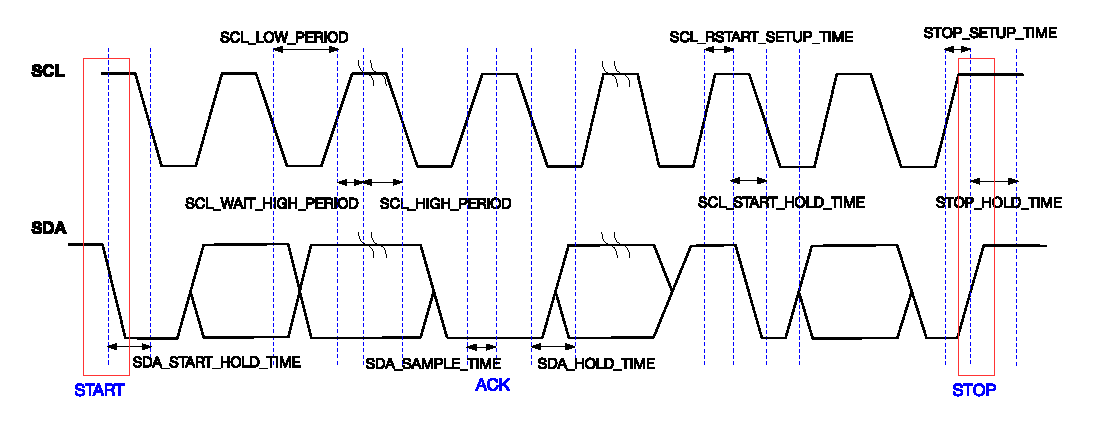
\includegraphics[width=0.9\textwidth]{\modulefiles/figures/I2C_bus_timing_723}
    \caption{I2C 时序图}
    \label{fig:i2c-bus-timing}
\end{figure}

图 \ref{fig:i2c-bus-timing} 为实现 I2C 协议的 I2C 主机的时序图,图中的寄存器均用来配置时序参数。I2C 控制器的 START 位、STOP 位、数据保持时间、数据采样时间、SCL 上升沿等待时间等时序均可以通过图 \ref{fig:i2c-bus-timing} 中所示的寄存器进行配置。这些寄存器以模块时钟 (I2C\_SCLK)  为单位,与各时序参数的对应关系为:

\begin{enumerate}
\item  $t_{LOW} = (\hyperref[fielddesc:I2CSCLLOWPERIOD]{I2C\_SCL\_LOW\_PERIOD} + 1) \cdot  T_{I2C\_SCLK}$

\item  $t_{HIGH} = (\hyperref[fielddesc:I2CSCLHIGHPERIOD]{I2C\_SCL\_HIGH\_PERIOD} + 1) \cdot  T_{I2C\_SCLK}$

\item  $t_{SU:STA} = (\hyperref[fielddesc:I2CSCLRSTARTSETUPTIME]{I2C\_SCL\_RSTART\_SETUP\_TIME} + 1) \cdot  T_{I2C\_SCLK}$

\item  $t_{HD:STA} = (\hyperref[fielddesc:I2CSCLSTARTHOLDTIME]{I2C\_SCL\_START\_HOLD\_TIME} +1) \cdot  T_{I2C\_SCLK}$

\item  $t_{r} = (\hyperref[fielddesc:I2CSCLWAITHIGHPERIOD]{I2C\_SCL\_WAIT\_HIGH\_PERIOD} + 1 ) \cdot  T_{I2C\_SCLK}$

\item  $t_{SU:STO} = (\hyperref[fielddesc:I2CSCLSTOPSETUPTIME]{I2C\_SCL\_STOP\_SETUP\_TIME}  + 1) \cdot  T_{I2C\_SCLK}$

\item  $t_{BUF} = (\hyperref[fielddesc:I2CSCLSTOPHOLDTIME]{I2C\_SCL\_STOP\_HOLD\_TIME}  + 1) \cdot  T_{I2C\_SCLK}$

\item  $t_{HD:DAT} = (\hyperref[fielddesc:I2CSDAHOLDTIME]{I2C\_SDA\_HOLD\_TIME} +1) \cdot  T_{I2C\_SCLK}$

\item  $t_{SU:DAT} = (\hyperref[fielddesc:I2CSCLLOWPERIOD]{I2C\_SCL\_LOW\_PERIOD} - \hyperref[fielddesc:I2CSDAHOLDTIME]{I2C\_SDA\_HOLD\_TIME}) \cdot  T_{I2C\_SCLK}$
\end{enumerate}

根据在何种模式下有意义,下列时序寄存器可分为两组:

\begin{itemize}

\item 主机模式:

\begin{enumerate}
\item \hyperref[fielddesc:I2CSCLSTARTHOLDTIME]{I2C\_SCL\_START\_HOLD\_TIME}:生成 I2C 协议中的 start 位时,SDA 信号拉低到 SCL 信号拉低的时间间隔。该时间间隔为 (\hyperref[fielddesc:I2CSCLSTARTHOLDTIME]{I2C\_SCL\_START\_HOLD\_TIME} +1)个模块时钟周期。仅控制器工作在主机模式时有意义。

\item \hyperref[fielddesc:I2CSCLLOWPERIOD]{I2C\_SCL\_LOW\_PERIOD}:SCL 低电平持续时间。SCL 低电平时间为 (\hyperref[fielddesc:I2CSCLLOWPERIOD]{I2C\_SCL\_LOW\_PERIOD} + 1) 个模块时钟周期。但是 如果外设拉低 SCL ,I2C 控制器执行 END 命令拉低 SCL,或者控制器发生 SCL时钟拉伸则可能会导致 SCL 低电平时间变长。仅控制器工作在主机模式时有意义。

\item \hyperref[fielddesc:I2CSCLWAITHIGHPERIOD]{I2C\_SCL\_WAIT\_HIGH\_PERIOD}:等待 SCL 线拉高的模块时钟周期数。请确保在该时间内 SCL 线可以完成上拉。否则会导致 SCL 高电平持续时间不可预测。仅控制器工作在主机模式时有意义。

\item \hyperref[fielddesc:I2CSCLHIGHPERIOD]{I2C\_SCL\_HIGH\_PERIOD}:SCL 线拉高后维持高电平的模块时钟周期数。仅控制器工作在主机模式时有意义。
当 SCL 线在 \hyperref[fielddesc:I2CSCLWAITHIGHPERIOD]{I2C\_SCL\_WAIT\_HIGH\_PERIOD} + 1 个模块时钟内完成上拉,则 SCL 线的频率为:
\[
    f_{scl}=\frac{f_{\textrm{I2C\_SCLK}}}
    {\textrm{\hyperref[fielddesc:I2CSCLLOWPERIOD]{I2C\_SCL\_LOW\_PERIOD} + \hyperref[fielddesc:I2CSCLHIGHPERIOD]{I2C\_SCL\_HIGH\_PERIOD} + \hyperref[fielddesc:I2CSCLWAITHIGHPERIOD]{I2C\_SCL\_WAIT\_HIGH\_PERIOD}+3}}
\]

\end{enumerate}

\item 主机模式和从机模式:

\begin{enumerate}

\item \hyperref[fielddesc:I2CSDASAMPLETIME]{I2C\_SDA\_SAMPLE\_TIME}:SCL 上升沿到采样 SDA 线电平值的时间间隔。推荐设置在 SCL 高电平持续时间的中间值,以保证能够正确采样到 SDA 线上电平。控制器工作在主机模式及从机模式时都有意义。

\item \hyperref[fielddesc:I2CSDAHOLDTIME]{I2C\_SDA\_HOLD\_TIME}:SDA 输出数据变化与 SCL 下降沿的时间间隔。控制器工作在主机模式及从机模式时都有意义。

\end{enumerate}

\end{itemize}

根据时序参数的限制,对时序寄存器的配置范围也有约束。
\begin{enumerate}
\item $\frac{f_{I2C\_SCLK}}{f_{SCL}} > 20$
\item $3 \times f_{I2C\_SCLK} \leq (\hyperref[fielddesc:I2CSDAHOLDTIME]{I2C\_SDA\_HOLD\_TIME}-4) \times f_{APB\_CLK}$
\item \hyperref[fielddesc:I2CSDAHOLDTIME]{I2C\_SDA\_HOLD\_TIME} + \hyperref[fielddesc:I2CSCLSTARTHOLDTIME]{I2C\_SCL\_START\_HOLD\_TIME} > SDA\_FILTER\_THRES + 3
\item \hyperref[fielddesc:I2CSCLWAITHIGHPERIOD]{I2C\_SCL\_WAIT\_HIGH\_PERIOD} < \hyperref[fielddesc:I2CSDASAMPLETIME]{I2C\_SDA\_SAMPLE\_TIME} < \hyperref[fielddesc:I2CSCLHIGHPERIOD]{I2C\_SCL\_HIGH\_PERIOD}
\item \hyperref[fielddesc:I2CSDASAMPLETIME]{I2C\_SDA\_SAMPLE\_TIME} < \hyperref[fielddesc:I2CSCLWAITHIGHPERIOD]{I2C\_SCL\_WAIT\_HIGH\_PERIOD} + \hyperref[fielddesc:I2CSCLSTARTHOLDTIME]{I2C\_SCL\_START\_HOLD\_TIME} +

\hyperref[fielddesc:I2CSCLRSTARTSETUPTIME]{I2C\_SCL\_RSTART\_SETUP\_TIME}
\item \hyperref[fielddesc:I2CSTRETCHPROTECTNUM]{I2C\_STRETCH\_PROTECT\_NUM} + \hyperref[fielddesc:I2CSDAHOLDTIME]{I2C\_SDA\_HOLD\_TIME} > \hyperref[fielddesc:I2CSCLLOWPERIOD]{I2C\_SCL\_LOW\_PERIOD}
\end{enumerate}

\subsection{超时控制}
I2C 内部有三种超时控制,分别是对 SCL\_FSM 状态的超时控制、SCL\_MAIN\_FSM 状态的超时控制和对SCL线状态的超时控制。其中前两种是一直打开的,第三种是可编程配置的。

当 SCL\_FSM 长时间处于同一状态不变,且时间超过 2$^{\hyperref[fielddesc:I2CSCLSTTOI2C]{I2C\_SCL\_ST\_TO\_I2C}}$ 个时钟周期后,会触发 I2C\_SCL\_ST\_TO\_INT 中断,状态机会回到空闲状态。\hyperref[fielddesc:I2CSCLSTTOI2C]{I2C\_SCL\_ST\_TO\_I2C}的配置值最大为 22,即最大在时间超过 2$^{22}$ 个 I2C\_SCLK 时钟周期后会产生超时中断。

当 SCL\_MAIN\_FSM 长时间处于同一状态不变,且时间超过 2$^{ \hyperref[fielddesc:I2CSCLMAINSTTOI2C]{I2C\_SCL\_MAIN\_ST\_TO\_I2C} }$ 个 I2C\_SCLK 时钟周期后,会触发 I2C\_SCL\_MAIN\_ST\_TO\_INT 中断,状态机会回到空闲状态。\hyperref[fielddesc:I2CSCLMAINSTTOI2C]{I2C\_SCL\_MAIN\_ST\_TO\_I2C} 的配置值最大为 22,即最大在时间超过 2$^{22}$ 个模块时钟后会产生超时中断。

使能 \hyperref[fielddesc:I2CTIMEOUTEN]{I2C\_TIME\_OUT\_EN} 打开 SCL 线状态的超时控制。当SCL线状态长时间维持同一电平不变,且时间超过 2$^{\hyperref[fielddesc:I2CTIMEOUTVALUE]{I2C\_TIME\_OUT\_VALUE}}$ 后,会触发 I2C\_TIME\_OUT\_INT 中断,I2C 总线回到空闲状态。

\subsection{指令配置}\label{sec:i2c-func-descr-cmd-controller}
I2C 控制器工作于主机模式时,CMD\_Controller 会依次从八个命令寄存器中读出命令并按照命令来控制 SCL\_FSM 及 SCL\_MAIN\_FSM。

\begin{figure}[H]
    \centering
    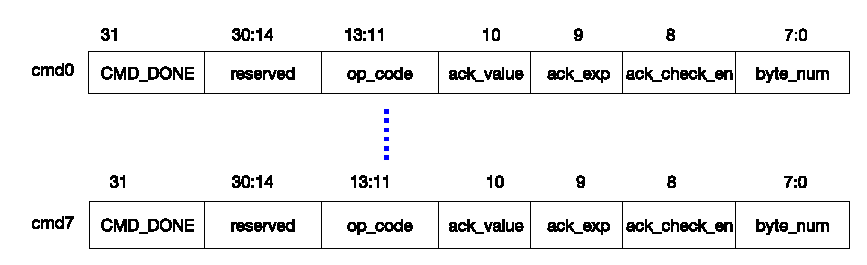
\includegraphics[width=0.8\textwidth]{\modulefiles/figures/I2C_Cmd_structure}
    \caption{I2C 命令寄存器结构}
    \label{fig:i2c-cmd-structure}
\end{figure}

命令寄存器只在 I2C 控制器工作于主机模式时才有效,其内部结构如图 \ref{fig:i2c-cmd-structure} 所示。命令寄存器的参数为:

\begin{enumerate}

\item CMD\_DONE: 命令执行完成标识。每条命令执行完硬件会将对应命令寄存器中的 CMD\_DONE 置 1。软件可以通过读取每条命令的 CMD\_DONE 位来判断该命令是否执行完毕。每次更新命令时,软件需要将 CMD\_DONE 位清零。

\item op\_code: 命令编码,共有五种命令:

\begin{itemize}
    \item RSTART: op\_code 等于 6 时为 RSTART 命令,该命令指示 I2C 控制器发送 I2C 协议中的 START 位或 RESTART 位。

    \item WRITE: op\_code 等于 1 时为 WRITE 命令,该命令指示 I2C 控制器向从机发送从机地址、被访问的寄存器地址(仅限双寻址模式)、数据。

    \item READ: op\_code 等于 3 时为 READ 命令,该命令指示 I2C 控制器从从机读取数据。

    \item STOP: op\_code 等于 2 时为 STOP 命令,该命令指示 I2C 控制器发送 I2C 协议中的 STOP 位。 此条命令也标识本次命令序列执行完成,CMD\_Controller 将会停止取指令。软件再次启动 CMD\_Controller 后,会重新从命令寄存器 0 开始去取指令。

    \item END: op\_code 等于 4 时为 END 命令,该命令指示 I2C 控制器将 SCL 信号拉低,暂停 I2C 通信。该命令也标识本次命令序列执行完成,CMD\_Controller 将会停止取指令。软件在更新命令寄存器和 RAM 数据后可重新启动 CMD\_Controller,继续进行 I2C 协议传输。再次启动后 CMD\_Controller 会重新从命令寄存器 0 开始去取指令。

\end{itemize}

\item ack\_value: 该位设置读操作时 I2C 控制器在 I2C 协议中的 ACK 位发送的电平值。 RSTART、STOP、END、WRITE 命令中该位没有意义。

\item ack\_exp: 该位用于设置写操作时 I2C 控制器在 I2C 协议中的 ACK 位期望接收的电平值。 RSTART、STOP、END、READ 命令中该位没有意义。

\item ack\_check\_en: 该位使能写操作中 I2C 控制器检查从机发送的 ACK 位电平与命令中的 ack\_exp 是否一致。如果接收的 ACK 值与 WRITE 命令中的 ack\_exp 电平不一致时,I2C 主机会产生 I2C\_NACK\_INT\\ 中断,停止发送数据并产生 STOP。 此位为 1 时,检测从机发送的 ACK 位电平;此位为 0 时,不检测从机发送的 ACK 位电平。RSTART、STOP、END、READ 命令中该位没有意义。

\item byte\_num: 读写数据的长度(单位字节),最大为 255,最小为 1。RSTART、STOP、END 命令中 byte\_num 无意义。

\end{enumerate}

每次命令序列的执行都是从命令寄存器 0 开始,到 STOP 或 END 命令结束。所以需要保证每个命令序列中必须有 STOP 或 END 命令。

一次完整的 I2C 协议传输应该起始于 START 命令,结束于 STOP 命令。可通过 END 命令将一次 I2C 协议传输分为多个命令序列来完成。每个命令序列可以改变数据传输的方向、时钟频率、从机地址和数据长度等。这样可以弥补 RAM 大小不足的问题,也可以实现更灵活的 I2C 通信。

\subsection{TX/RX RAM数据存储}
\label{subsubsec:i2c-txrx}
TX/RX RAM大小均为 32 x 8 位。 TX RAM 和 RX RAM 均可以通过 FIFO 和直接地址 (non-FIFO) 两种方式访问。将 \hyperref[fielddesc:I2CNONFIFOEN]{I2C\_NONFIFO\_EN} 位设置成 0,为 FIFO 方式;\hyperref[fielddesc:I2CNONFIFOEN]{I2C\_NONFIFO\_EN} 位设置成 1 时为直接地址方式。

TX RAM 用于存储 I2C 控制器需要发送的数据。在 I2C 通信的过程中,当 I2C 控制器需要发送数据时(不包括 ACK 位响应),会依次读出 TX RAM 中的数据并串行输出到 SDA 线上。当 I2C 控制器工作于主机模式时,所有需要发送给从机的数据都必须按照发送顺序依次存储在 TX RAM 中。包括被访问的从机地址、读写标志位、被访问的寄存器地址(仅限双地址寻址模式下)、写数据。当 I2C 控制器工作于从机模式时,TX RAM 中只存放写数据。

TX RAM 可被 CPU 读写。CPU 可通过两种方式写 TX RAM: FIFO 访问和直接地址访问。FIFO 访问方式是通过固定地址 \hyperref[regdesc:I2CDATAREG]{I2C\_DATA\_REG} 写 TX RAM,硬件自动进行 TX RAM 写地址自增。直接地址访问是通过地址段 (\hyperref[tab:sysmem-base-address]{I2C 基地址} + 0x{}100) \textasciitilde (\hyperref[tab:sysmem-base-address]{I2C 基地址} + 0x{}17C) 直接访问 TX RAM。TX RAM 的每一个字节占据一个字 (word) 的地址。因此,第一个字节访问地址为 \hyperref[tab:sysmem-base-address]{I2C 基地址} + 0x{}100,第二字节访问地址为 \hyperref[tab:sysmem-base-address]{I2C 基地址} + 0x{}104,第三字节访问地址为 \hyperref[tab:sysmem-base-address]{I2C 基地址} + 0x{}108,以此类推。CPU 只可通过直接地址访问方式读 TX RAM,读 TX RAM 的地址和写 TX RAM 的地址相同。

RX RAM 存储的是 I2C 通信过程中,I2C 控制器接收到的数据。当I2C 控制器工作于从机模式时,主机发送的从机地址及被访问的寄存器地址(仅限双地址寻址模式下)都不会存储在 RX RAM 中。软件可以在 I2C 通信结束后,读出 RX RAM 的值。


RX RAM 只可被 CPU 读。CPU 可通过两种方式读 RX RAM: FIFO 访问和直接地址访问。FIFO 访问方式是通过固定地址 \hyperref[regdesc:I2CDATAREG]{I2C\_DATA\_REG} 读 RX RAM,硬件自动完成 RX RAM 读地址自增。直接地址访问是通过地址段 (\hyperref[tab:sysmem-base-address]{I2C 基地址} + 0x{}180) \textasciitilde (\hyperref[tab:sysmem-base-address]{I2C 基地址} + 0x{}1FC) 直接访问 RX RAM。RX RAM 的每一个字节占据一个字的地址。因此,第一个字节访问地址为 \hyperref[tab:sysmem-base-address]{I2C 基地址} + 0x{}180,第二字节访问地址为 \hyperref[tab:sysmem-base-address]{I2C 基地址} + 0x{}184,第三字节访问地址为 \hyperref[tab:sysmem-base-address]{I2C 基地址} + 0x{}188,以此类推。

在 FIFO 模式下可以对 TX RAM 进行乒乓操作,来实现发送大于 32 个字节的数据。置位 \hyperref[fielddesc:I2CFIFOPRTEN]{I2C\_FIFO\_PRT\_EN},当RAM 中剩下的待发送数据字节数小于 \hyperref[fielddesc:I2CTXFIFOWMTHRHD]{I2C\_TXFIFO\_WM\_THRHD}时,会产生 I2C\_TXFIFO\_WM\_INT 中断。软件收到中断后,继续向 \hyperref[regdesc:I2CDATAREG]{I2C\_DATA\_REG}(主机)中写数。需要保证向 TX RAM 写数或更新数据的操作提前于 I2C 发送数据的动作,否则会产生不可预计的后果。

在 FIFO 模式下也可以对 RX RAM 进行乒乓操作,来实现接收大于 32 个字节的数据。置位 \hyperref[fielddesc:I2CFIFOPRTEN]{I2C\_FIFO\_PRT\_EN},将 \hyperref[fielddesc:I2CRXFULLACKLEVEL]{I2C\_RX\_FULL\_ACK\_LEVEL} 置 0。当 RAM 中收到的数据字节数大于等于 \hyperref[fielddesc:I2CRXFIFOWMTHRHD]{I2C\_RXFIFO\_WM\_THRHD}(从机) 时,会产生 I2C\_RXFIFO\_WM\_INT 中断。软件收到中断后,从 \hyperref[regdesc:I2CDATAREG]{I2C\_DATA\_REG} (从机)中读数。

\subsection{数据转换}
DATA\_Shifter 模块用于串并转换,当 I2C 发送数据时,将 TX RAM 中的字节数据转化成比特流;当 I2C 接收数据时,将比特流转化成字节数据并存入 RX RAM。\hyperref[fielddesc:I2CRXLSBFIRST]{I2C\_RX\_LSB\_FIRST} 和 \hyperref[fielddesc:I2CTXLSBFIRST]{I2C\_TX\_LSB\_FIRST} 用于配置最高有效位或最低有效位的优先储存或传输。

\subsection{寻址模式}
除了 7 位寻址模式,\chipname{} I2C 还支持 10 位寻址模式和双寻址模式。10 位寻址和 7 位寻址可结合使用。

假设从机地址为 SLV\_ADDR 。 \chipname{} I2C 控制器可以使用 7 位寻址(SLV\_ADDR[6:0]),也可以使用 10 位寻址(SLV\_ADDR[9:0]) 。

对于主机模式而言,7 位寻址下只要发送一个字节地址段 SLV\_ADDR[6:0] 和读写标志。7位寻址模式下,有种特殊情况是广播寻址。在从机中,将 \hyperref[fielddesc:I2CADDRBROADCASTINGEN]{I2C\_ADDR\_BROADCASTING\_EN}置 1,开启广播寻址模式。当接收到主机发送的地址为广播地址(0x{}00)且读写标志位为0时,此时无论从机自己的地址是多少,都会响应主机。

10 位寻址需要发送两字节地址段。第一个要发送的数是从机地址的第一个 7 位 slave\_addr\_first\_7bits 和读写标志,slave\_addr\_first\_7bits 的值应该配置为 (0x{}78 | SLV\_ADDR[9:8])。第二个要发送的数是 slave\_addr\_second\_byte,slave\_addr\_second\_byte 的值为 SLV\_ADDR[7:0]。

在从机中,可以通过配置 \hyperref[fielddesc:I2CADDR10BITEN]{I2C\_ADDR\_10BIT\_EN} 寄存器开启 10 位寻址模式。 \hyperref[fielddesc:I2CSLAVEADDR]{I2C\_SLAVE\_ADDR} 用于配置 I2C 从机地址。\hyperref[fielddesc:I2CSLAVEADDR]{I2C\_SLAVE\_ADDR}[14:7] 的值应配置为 SLV\_ADDR[7:0],\hyperref[fielddesc:I2CSLAVEADDR]{I2C\_SLAVE\_ADDR}[6:0] 的值应配置为 (0x{}78 | SLV\_ADDR[9:8]) 。由于 10 位从机地址比 7 位地址多一个字节,所以 WRITE 命令对应的 byte\_num 以及 RAM 中数据数量都相应增加 1。

控制器处于从机模式时,还支持双地址访问方式。双地址的第一个地址是 I2C 从机地址,第二个地址是 I2C 从机的内存地址。双地址模式下,RAM 必须采用 non-FIFO 方式访问。
通过置位 \hyperref[fielddesc:I2CFIFOADDRCFGEN]{I2C\_FIFO\_ADDR\_CFG\_EN} 来使能双地址访问功能。

\subsection{10 位寻址的读写标志位检查}
在 10 位寻址模式下,将 \hyperref[fielddesc:I2CADDR10BITRWCHECKEN]{I2C\_ADDR\_10BIT\_RW\_CHECK\_EN} 置 1,会对发送的第一个数slave\_addr\_first\_7bits 和读写标志做检查。当读写标志不是写,此时与协议不符合,会结束传输。若不打开此功能,当读写标志不是写,还能支持继续传输,但可能出现传输错误。

\subsection{启动控制器}
\label{subsubsec:i2c-start}
对于主机,配置成主机模式和命令寄存器等相关配置后,通过向 \hyperref[fielddesc:I2CTRANSSTART]{I2C\_TRANS\_START} 写 1,启动主机解析,执行命令序列。一组命令总是从命令寄存器 0 开始,顺序执行到 STOP 或者 END 命令。当另一组命令需要从命令寄存器 0 开始执行时,需要重新向 \hyperref[fielddesc:I2CTRANSSTART]{I2C\_TRANS\_START} 写 1 来更新命令。

对于从机,有两种启动方式:
\begin{itemize}
    \item 置位 \hyperref[fielddesc:I2CSLVTXAUTOSTARTEN]{I2C\_SLV\_TX\_AUTO\_START\_EN},则从机会在被主机寻址后自动启动传输;
    \item 清零 \hyperref[fielddesc:I2CSLVTXAUTOSTARTEN]{I2C\_SLV\_TX\_AUTO\_START\_EN},且在每次传输前必须置位 \hyperref[fielddesc:I2CTRANSSTART]{I2C\_TRANS\_START}。
\end{itemize}

\section{编程示例}
本节提供一些典型通信场景的编程示例。\chipname{}中有两个 I2C 外设控制器,为了便于描述,下文所有图示中的 I2C 主机和从机都假定为\chipname{} I2C 外设控制器。

\subsection{I2C 主机写入从机,7 位寻址,单次命令序列}\label{subsec:i2c-mws7}
\subsubsection{场景介绍}
\begin{figure}[H]
    \centering
    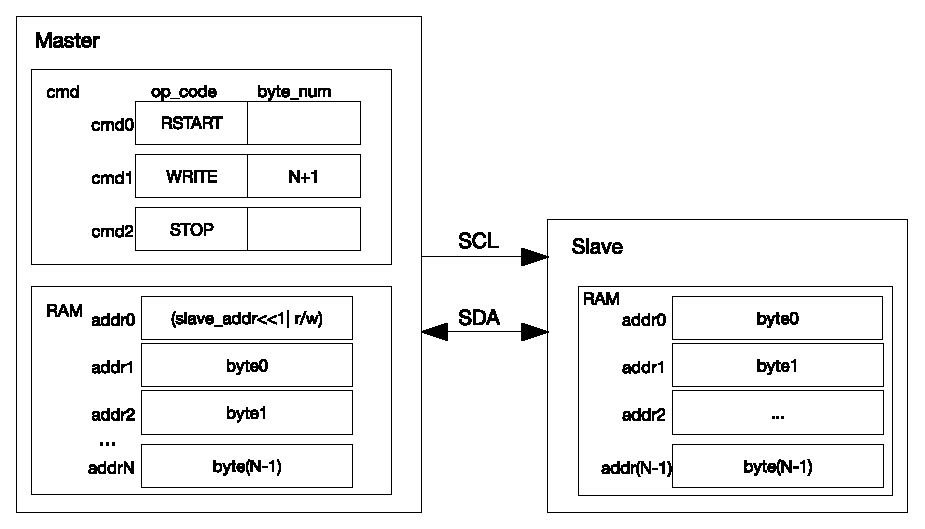
\includegraphics[width=0.8\textwidth]{\modulefiles/figures/I2C_MWS7}
    \caption{I2C 主机写 7 位寻址的从机}
    \label{fig:i2c-mws7}
\end{figure}

图 \ref{fig:i2c-mws7} 为 I2C 主机采用 7 位寻址写 N 个字节数据到 I2C 从机的寄存器或 RAM。如图 \ref{fig:i2c-mws7} 所示,主机 RAM 中第一个字节数据为 7 位从机地址 + 1 位读写标志位,其中读写标志位为 0 时表示写操作,接下来的连续空间存储待发送的数据。cmd 框中包含了相应的命令序列。

对于主机,在软件配置好命令序列以及 RAM 数据后,置位 \hyperref[fielddesc:I2CTRANSSTART]{I2C\_TRANS\_START} 寄存器启动控制器进行数据传输。控制器的行为可分为四步:
\begin{enumerate}
    \item 等待 SCL 线为高电平,以避免 SCL 线被其他 主机或者 从机占用。
    \item 执行 RSTART 命令发送 START 位。
    \item 执行 WRITE 命令从 RAM 的首地址开始取出 N+1 个字节并依次发送给从机,其中第一个字节为地址。
    \item 发送 STOP。当 I2C 主机完成 STOP 位的传输后,会产生 I2C\_TRANS\_COMPLETE\_INT 中断。
\end{enumerate}

\subsubsection{配置示例}
\begin{enumerate}
\item 参照章节 \ref{subsec:i2c-timing-para},配置 I2C 主机和 I2C 从机的时序参数寄存器。
\item 设置 \hyperref[fielddesc:I2CMSMODE]{I2C\_MS\_MODE}(主机)为1,\hyperref[fielddesc:I2CMSMODE]{I2C\_MS\_MODE}(从机)为0。
\item 向 \hyperref[fielddesc:I2CCONFUPGATE]{I2C\_CONF\_UPGATE}(主机)和 \hyperref[fielddesc:I2CCONFUPGATE]{I2C\_CONF\_UPGATE}(从机)写1来同步寄存器。
\clearpage
\item 配置 I2C 主机的指令寄存器。

\begin{longtable}{ | p{4cm} | p{2cm} | p{2cm} | p{2cm} |p{2cm} | p{2cm} |}
\hline\rowcolor{lightgray}
指令寄存器& op\_code & ack\_value&ack\_exp&ack\_check\_en&byte\_num  \\ \hline
\hyperref[fielddesc:I2CCOMMAND0]{I2C\_COMMAND0}(主机)& RSTART& ---&---&---&---  \\ \hline
\hyperref[fielddesc:I2CCOMMAND1]{I2C\_COMMAND1}(主机)& WRITE& ack\_value&ack\_exp&1&N+1  \\ \hline
\hyperref[fielddesc:I2CCOMMAND2]{I2C\_COMMAND2}(主机)& STOP& ---&---&---&---  \\ \hline
\end{longtable}

\item 参考章节 \ref{subsubsec:i2c-txrx},向 I2C 主机的 TX RAM 写入从机地址和要发送的数据。可选FIFO方式和直接访问方式。
\item 在 \hyperref[regdesc:I2CSLAVEADDRREG]{I2C\_SLAVE\_ADDR\_REG}(从机)的 \hyperref[fielddesc:I2CSLAVEADDR]{I2C\_SLAVE\_ADDR}(从机)设置 I2C 从机的地址。
\item 向 \hyperref[fielddesc:I2CCONFUPGATE]{I2C\_CONF\_UPGATE}(主机)和 \hyperref[fielddesc:I2CCONFUPGATE]{I2C\_CONF\_UPGATE}(从机)写 1 来同步寄存器。
\item 向 \hyperref[fielddesc:I2CTRANSSTART]{I2C\_TRANS\_START}(主机)和 \hyperref[fielddesc:I2CTRANSSTART]{I2C\_TRANS\_START}(从机)位写 1 开始传输。
\item I2C 从机比较 I2C 主机发送的从机地址和自己的 \hyperref[fielddesc:I2CSLAVEADDR]{I2C\_SLAVE\_ADDR}(从机),当 I2C 主机 WRITE 命令中的 ack\_check\_en(主机)配置为 1 时,I2C 主机会在发送完每个字节之后进行 ACK 检测。 若 ack\_check\_en 配置为 0,则不会对 ACK 检测,会默认为匹配。
\begin{itemize}
\item 匹配:接收的 ACK 值与 WRITE 命令中的 ack\_exp(主机) 电平一致,传输继续。
\item 不匹配:接收的 ACK 值与 WRITE 命令中的 ack\_exp(主机) 电平不一致,I2C 主机产生 I2C\_NACK\_INT(主机) 中断,停止发送数据并且产生 STOP。
\end{itemize}

\item I2C 主机发送数据,并根据 ack\_check\_en(主机) 配置的不同进行或不进行 ACK 检测。
\item 若发送数据 N 大于 32 字节,在 FIFO 模式下可以对 I2C 主机的 TX RAM 进行乒乓操作,具体做法参照章节 \ref{subsubsec:i2c-txrx}。
\item 若接收数据 N 大于32 字节,在 FIFO 模式下可以对 I2C 从机的RX RAM进行乒乓操作,具体做法参照章节 \ref{subsubsec:i2c-txrx}。

若接收数据 N 大于32 字节,另一种处理方式是置位 \hyperref[fielddesc:I2CSLAVESCLSTRETCHEN]{I2C\_SLAVE\_SCL\_STRETCH\_EN}(从机)使能 SCL 时钟拉伸,同时将 \hyperref[fielddesc:I2CRXFULLACKLEVEL]{I2C\_RX\_FULL\_ACK\_LEVEL} 置 0。RX RAM 满时会产生 \hyperref[int:i2c-slave-stretch]{I2C\_SLAVE\_STRETCH\_INT}(从机)中断。此时 I2C 从机会将 SCL 拉低,软件在此期间可以读取数据。等完成操作后再将 \hyperref[fielddesc:I2CSLAVESTRETCHINTCLR]{I2C\_SLAVE\_STRETCH\_INT\_CLR}(从机)置 1 清除中断,并将\hyperref[fielddesc:I2CSLAVESCLSTRETCHCLR]{I2C\_SLAVE\_SCL\_STRETCH\_CLR}(从机)置1 释放 SCL 总线。
\item 当整个传输正常结束,I2C 主机执行 STOP 命令,并产生 I2C\_TRANS\_COMPLETE\_INT(主机) 中断。

\end{enumerate}




\subsection{I2C 主机写入从机,10 位寻址,单次命令序列}\label{sub:i2c-app-mws10}
\subsubsection{场景介绍}
\begin{figure}[H]
    \centering
    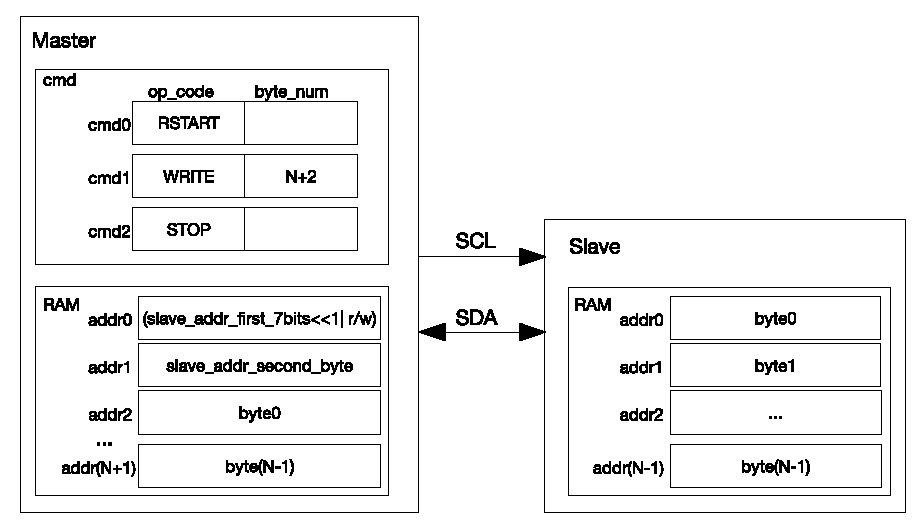
\includegraphics[width=0.8\textwidth]{\modulefiles/figures/I2C_MWS10}
    \caption{I2C 主机写 10 位寻址的从机}
    \label{fig:i2c-mws10}
\end{figure}


图 \ref{fig:i2c-mws10} 为 I2C 主机写 N 个字节到 10 位地址 I2C 从机的配置图。整个配置和传输过程都和 \ref{subsec:i2c-mws7}中类似,除了在传输的开始主机在10位寻址模式下需要发送两字节地址段。由于 10 位从机地址比 7 位地址多一个字节,所以 WRITE 命令对应的 byte\_num 以及TX RAM 中数据数量都相应增加 1。

\subsubsection{配置示例}
\begin{enumerate}
\item 设置 \hyperref[fielddesc:I2CMSMODE]{I2C\_MS\_MODE}(主机)为1,\hyperref[fielddesc:I2CMSMODE]{I2C\_MS\_MODE}(从机)为0。
\item 向 \hyperref[fielddesc:I2CCONFUPGATE]{I2C\_CONF\_UPGATE}(主机)和 \hyperref[fielddesc:I2CCONFUPGATE]{I2C\_CONF\_UPGATE}(从机)写 1 来同步寄存器。
\item 配置 I2C 主机的指令寄存器。

\begin{longtable}{ | p{4cm} | p{2cm} | p{2cm} | p{2cm} |p{2cm} | p{2cm} |}
\hline\rowcolor{lightgray}
指令寄存器& op\_code & ack\_value&ack\_exp&ack\_check\_en&byte\_num  \\ \hline
\hyperref[fielddesc:I2CCOMMAND0]{I2C\_COMMAND0}(主机)& RSTART& ---&---&---&---  \\ \hline
\hyperref[fielddesc:I2CCOMMAND1]{I2C\_COMMAND1}(主机)& WRITE& ack\_value&ack\_exp&1&N+2  \\ \hline
\hyperref[fielddesc:I2CCOMMAND2]{I2C\_COMMAND2}(主机)& STOP& ---&---&---&---  \\ \hline
\end{longtable}

\item 在 \hyperref[regdesc:I2CSLAVEADDRREG]{I2C\_SLAVE\_ADDR\_REG}(从机)的 \hyperref[fielddesc:I2CSLAVEADDR]{I2C\_SLAVE\_ADDR}(从机)设置 I2C 从机的 10 位从机地址,并将 \hyperref[fielddesc:I2CADDR10BITEN]{I2C\_ADDR\_10BIT\_EN}(从机)置 1 使能 10 位寻址模式。
\item 向 I2C 主机的TX RAM写入从机地址和要发送的数据,第一个地址字节是((0x{}78 | \hyperref[fielddesc:I2CSLAVEADDR]{I2C\_SLAVE\_ADDR}[9:8])<<1)|R/W,第二个地址字节是\hyperref[fielddesc:I2CSLAVEADDR]{I2C\_SLAVE\_ADDR}[7:0]。之后就是要发送的数据,可选FIFO方式和直接访问方式。
\item 向 \hyperref[fielddesc:I2CCONFUPGATE]{I2C\_CONF\_UPGATE}(主机)和 \hyperref[fielddesc:I2CCONFUPGATE]{I2C\_CONF\_UPGATE}(从机)写1来同步寄存器。
\item 向 \hyperref[fielddesc:I2CTRANSSTART]{I2C\_TRANS\_START}(主机)和 \hyperref[fielddesc:I2CTRANSSTART]{I2C\_TRANS\_START}(从机)位写1开始传输。
\item I2C 从机比较 I2C 主机发送的从机地址和自己的\hyperref[fielddesc:I2CSLAVEADDR]{I2C\_SLAVE\_ADDR}(从机),当 I2C 主机 WRITE 命令中的 ack\_check\_en(主机) 配置为 1 时,I2C 主机会在发送完每个字节之后进行 ACK 检测。 若ack\_check\_en 配置为 0,则不会对ACK检测,会默认为匹配。
\begin{itemize}
\item 匹配:接收的 ACK 值与 WRITE 命令中的 ack\_exp(主机) 电平一致,传输继续。
\item 不匹配:接收的 ACK 值与 WRITE 命令中的 ack\_exp(主机) 电平不一致,I2C 主机产生 I2C\_NACK\_INT(主机) 中断,停止发送数据并且产生 STOP。
\end{itemize}

\item I2C 主机发送数据,并根据ack\_check\_en(主机) 配置的不同进行或不进行ACK检测。

\item 若发送数据 N 大于 32 字节,在 FIFO 模式下可以对 I2C 主机的 TX RAM 进行乒乓操作,具体做法参照章节 \ref{subsubsec:i2c-txrx}。
\item 若接收数据 N 大于32 字节,在 FIFO 模式下可以对 I2C 从机的RX RAM进行乒乓操作,具体做法参照章节 \ref{subsubsec:i2c-txrx}。

若接收数据 N 大于32 字节,另一种处理方式是置位 \hyperref[fielddesc:I2CSLAVESCLSTRETCHEN]{I2C\_SLAVE\_SCL\_STRETCH\_EN}(从机)使能 SCL 时钟拉伸,同时将 \hyperref[fielddesc:I2CRXFULLACKLEVEL]{I2C\_RX\_FULL\_ACK\_LEVEL} 置 0。RX RAM 满时会产生 \hyperref[int:i2c-slave-stretch]{I2C\_SLAVE\_STRETCH\_INT}(从机)中断。此时 I2C 从机会将 SCL 拉低,软件在此期间可以读取数据。等完成操作后再将 \hyperref[fielddesc:I2CSLAVESTRETCHINTCLR]{I2C\_SLAVE\_STRETCH\_INT\_CLR}(从机)置 1 清除中断,并将\hyperref[fielddesc:I2CSLAVESCLSTRETCHCLR]{I2C\_SLAVE\_SCL\_STRETCH\_CLR}(从机)置1 释放 SCL 总线。

\item 当整个传输正常结束,I2C 主机执行STOP命令,并产生 I2C\_TRANS\_COMPLETE\_INT(主机) 中断。

\end{enumerate}



\subsection{I2C 主机写入从机,7 位双地址寻址,单次命令序列}
\subsubsection{场景介绍}
\begin{figure}[H]
    \centering
    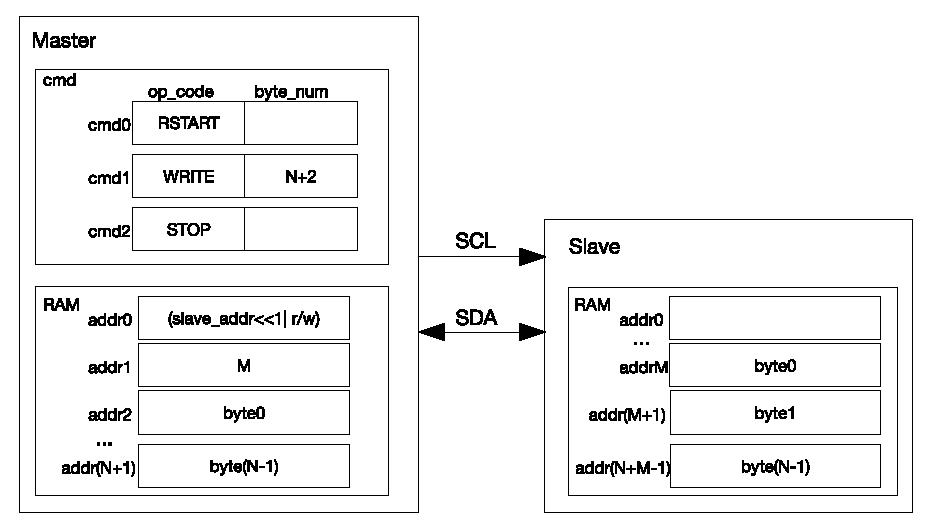
\includegraphics[width=0.8\textwidth]{\modulefiles/figures/I2C_MWS7_M}
    \caption{I2C 主机写 7 位双地址寻址从机}
    \label{fig:i2c-mws7-double}
\end{figure}

图\ref{fig:i2c-mws7-double} 为I2C主机采用7位双寻址模式写N个字节数据到I2C从机的寄存器或 RAM 的值。整个配置和传输过程都和章节 \ref{subsec:i2c-mws7} 中类似,区别是传输的开始主机在 7 位双寻址模式下需要发送两个字节。双地址的第一个地址是 7 位从机地址,第二个地址是 I2C 从机的内存地址(即图 \ref{fig:i2c-mws7-double} 中的 addrM)。双地址模式下,RX RAM 必须采用 non-FIFO 方式访问。另一个区别是,I2C 从机将接收到的数据 byte0 \verb+~+ byte(N-1) 从 RX RAM 中的 addrM 开始依次存储,addrM就是主机发送的I2C内存地址。当超出地址 31 后会从地址0开始继续存储。


\subsubsection{配置示例}
\begin{enumerate}
\item 设置 \hyperref[fielddesc:I2CMSMODE]{I2C\_MS\_MODE}(主机)为1,\hyperref[fielddesc:I2CMSMODE]{I2C\_MS\_MODE}(从机)为0。
\item 设置\hyperref[fielddesc:I2CFIFOADDRCFGEN]{I2C\_FIFO\_ADDR\_CFG\_EN}(从机)为1来使能双寻址模式。
\item 向 \hyperref[fielddesc:I2CCONFUPGATE]{I2C\_CONF\_UPGATE}(主机)和 \hyperref[fielddesc:I2CCONFUPGATE]{I2C\_CONF\_UPGATE}(从机)写1来同步寄存器。
\item 配置 I2C 主机的指令寄存器。
\begin{longtable}{ | p{4cm} | p{2cm} | p{2cm} | p{2cm} |p{2cm} | p{2cm} |}
\hline\rowcolor{lightgray}
指令寄存器& op\_code & ack\_value&ack\_exp&ack\_check\_en&byte\_num  \\ \hline
\hyperref[fielddesc:I2CCOMMAND0]{I2C\_COMMAND0}(主机)& RSTART& ---&---&---&---  \\ \hline
\hyperref[fielddesc:I2CCOMMAND1]{I2C\_COMMAND1}(主机)& WRITE& ack\_value&ack\_exp&1&N+2  \\ \hline
\hyperref[fielddesc:I2CCOMMAND2]{I2C\_COMMAND2}(主机)& STOP& ---&---&---&---  \\ \hline
\end{longtable}
\item 向 I2C 主机的TX RAM写入从机地址和要发送的数据,可以用FIFO方式或直接访问方式。
\item 在\hyperref[regdesc:I2CSLAVEADDRREG]{I2C\_SLAVE\_ADDR\_REG}(从机)的\hyperref[fielddesc:I2CSLAVEADDR]{I2C\_SLAVE\_ADDR}(从机)设置 I2C 从机的地址。
\item 向 \hyperref[fielddesc:I2CCONFUPGATE]{I2C\_CONF\_UPGATE}(主机)和 \hyperref[fielddesc:I2CCONFUPGATE]{I2C\_CONF\_UPGATE}(从机)写1来同步寄存器。
\item 向 \hyperref[fielddesc:I2CTRANSSTART]{I2C\_TRANS\_START}(主机)和 \hyperref[fielddesc:I2CTRANSSTART]{I2C\_TRANS\_START}(从机)位写1开始传输。
\item I2C 从机比较 I2C 主机发送的从机地址和自己的\hyperref[fielddesc:I2CSLAVEADDR]{I2C\_SLAVE\_ADDR}(从机),当 I2C 主机 WRITE 命令中的 ack\_check\_en(主机) 配置为 1 时,I2C 主机会在发送完每个字节之后进行 ACK 检测。 若ack\_check\_en 配置为 0,则不会对ACK检测,会默认为匹配。
\begin{itemize}
\item 匹配:接收的 ACK 值与 WRITE 命令中的 ack\_exp(主机) 电平一致,传输继续。
\item 不匹配:接收的 ACK 值与 WRITE 命令中的 ack\_exp(主机) 电平不一致,I2C 主机产生 I2C\_NACK\_INT(主机) 中断,停止发送数据并且产生 STOP。
\end{itemize}
\item I2C 从机接收到 I2C 主机发送的内存地址,完成RX RAM的地址偏移。

\item I2C 主机发送数据,并根据ack\_check\_en(主机)
配置的不同进行或不进行ACK检测。
\item 若发送数据 N 大于 32 字节,在 FIFO 模式下可以对 I2C 主机的 TX RAM 进行乒乓操作,具体做法参照章节 \ref{subsubsec:i2c-txrx}。
\item 若接收数据 N 大于32 字节,置位 \hyperref[fielddesc:I2CSLAVESCLSTRETCHEN]{I2C\_SLAVE\_SCL\_STRETCH\_EN}(从机)使能 SCL 时钟拉伸,同时将 \hyperref[fielddesc:I2CRXFULLACKLEVEL]{I2C\_RX\_FULL\_ACK\_LEVEL} 置 0。RX RAM 满时会产生 \hyperref[int:i2c-slave-stretch]{I2C\_SLAVE\_STRETCH\_INT}(从机)中断。此时 I2C 从机会将 SCL 拉低,软件在此期间可以读取数据。等完成操作后再将 \hyperref[fielddesc:I2CSLAVESTRETCHINTCLR]{I2C\_SLAVE\_STRETCH\_INT\_CLR}(从机)置 1 清除中断,并将\hyperref[fielddesc:I2CSLAVESCLSTRETCHCLR]{I2C\_SLAVE\_SCL\_STRETCH\_CLR}(从机)置1 释放 SCL 总线。

\item 当整个传输正常结束,I2C 主机执行STOP命令,并产生 I2C\_TRANS\_COMPLETE\_INT(主机) 中断。

\end{enumerate}

\subsection{I2C 主机写入从机,7 位寻址,多次命令序列}
\subsubsection{场景介绍}
\begin{figure}[H]
    \centering
    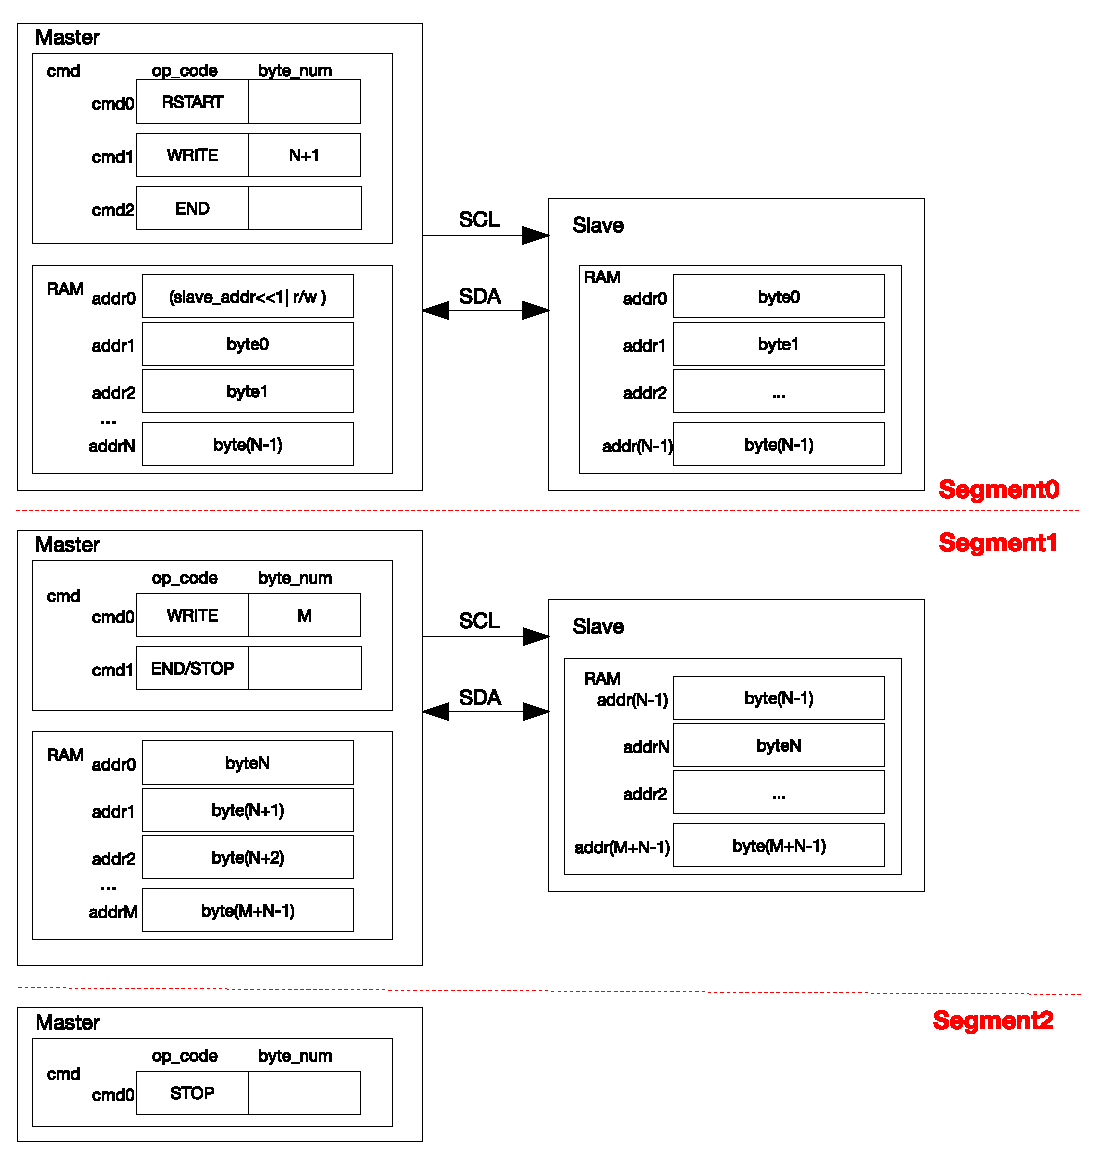
\includegraphics[width=0.8\textwidth]{\modulefiles/figures/I2C_MWS_END}    \caption{I2C 主机分段写 7 位寻址的从机}
    \label{fig:i2c-mws7-multiple}
\end{figure}

RAM 的大小只有 32 字节,对于大量的数据传输当 RAM 乒乓操作也不能满足要求时,建议使用多次命令序列进行分段传输。每次命令序列以 END 命令结尾,这样控制器会执行 END 命令拉低  SCL 线,软件此时可以更新命令序列寄存器和 RAM 的内容以用于下一次命令序列的传输。

以两段和三段传输为例,如图 \ref{fig:i2c-mws7-multiple} 所示为 I2C 主机分成三段或者两段写从机。配置 I2C 主机的命令序列如第一段所示,并且在 主机的 RAM 中准备好数据,置位 \hyperref[fielddesc:I2CTRANSSTART]{I2C\_TRANS\_START},I2C 主机即开始数据传输。 在执行到 END 命令后,I2C 主机会关闭 SCL 时钟,并将 SCL 线拉低来防止其他设备占用 I2C 总线。此时控制器产生 I2C\_END\_DETECT\_INT 中断。

在检测到 I2C\_END\_DETECT\_INT 中断后,软件可以更新命令序列 以及 RAM 中的内容如第二段所示,并清除 I2C\_END\_DETECT\_INT 中断。当第二段中 cmd1 为 STOP 时,不需要第三段,即为两段写从机。 置位 \hyperref[fielddesc:I2CTRANSSTART]{I2C\_TRANS\_START} 后,I2C 主机继续发送数据,并在最后发送 STOP 位。当为三段写 从机时,I2C 主机在第二段发送完数据,并检测到 I2C 主机的 I2C\_END\_DETECT\_INT 中断后,即可配置 cmd 如第三段所示。置位 \hyperref[fielddesc:I2CTRANSSTART]{I2C\_TRANS\_START} 后,I2C 主机即产生 STOP 位,从而停止传输。

请注意,在两个分段之间,I2C 总线上的其他 主机设备不会占用总线。 只有在发送了 STOP 信号后总线才会被释放。任何情况下,置位 \hyperref[fielddesc:I2CFSMRST]{I2C\_FSM\_RST} 可复位 I2C 控制器,硬件自清 \hyperref[fielddesc:I2CFSMRST]{I2C\_FSM\_RST}。

\subsubsection{配置示例}
\begin{enumerate}
\item 设置 \hyperref[fielddesc:I2CMSMODE]{I2C\_MS\_MODE}(主机)为1,\hyperref[fielddesc:I2CMSMODE]{I2C\_MS\_MODE}(从机)为0。
\item 向 \hyperref[fielddesc:I2CCONFUPGATE]{I2C\_CONF\_UPGATE}(主机)和 \hyperref[fielddesc:I2CCONFUPGATE]{I2C\_CONF\_UPGATE}(从机)写1来同步寄存器。
\item 配置 I2C 主机的指令寄存器。
\begin{longtable}{ | p{4cm} | p{2cm} | p{2cm} | p{2cm} |p{2cm} | p{2cm} |}
\hline\rowcolor{lightgray}
指令寄存器& op\_code & ack\_value&ack\_exp&ack\_check\_en&byte\_num  \\ \hline
\hyperref[fielddesc:I2CCOMMAND0]{I2C\_COMMAND0}(主机)& RSTART& ---&---&---&---  \\ \hline
\hyperref[fielddesc:I2CCOMMAND1]{I2C\_COMMAND1}(主机)& WRITE& ack\_value&ack\_exp&1&N+1  \\ \hline
\hyperref[fielddesc:I2CCOMMAND2]{I2C\_COMMAND2}(主机)& END& ---&---&---&---  \\ \hline
\end{longtable}
\item 参考章节 \ref{subsubsec:i2c-txrx},向 I2C 主机的TX RAM写入从机地址和要发送的数据。可选FIFO方式和直接访问方式。
\item 在\hyperref[regdesc:I2CSLAVEADDRREG]{I2C\_SLAVE\_ADDR\_REG}(从机)的\hyperref[fielddesc:I2CSLAVEADDR]{I2C\_SLAVE\_ADDR}(从机)设置 I2C 从机的地址。
\item 向 \hyperref[fielddesc:I2CCONFUPGATE]{I2C\_CONF\_UPGATE}(主机)和 \hyperref[fielddesc:I2CCONFUPGATE]{I2C\_CONF\_UPGATE}(从机)写1来同步寄存器。
\item 向 \hyperref[fielddesc:I2CTRANSSTART]{I2C\_TRANS\_START}(主机)和 \hyperref[fielddesc:I2CTRANSSTART]{I2C\_TRANS\_START}(从机)位写1开始传输。
\item I2C 从机比较 I2C 主机发送的从机地址和自己的\hyperref[fielddesc:I2CSLAVEADDR]{I2C\_SLAVE\_ADDR}(从机),当 I2C 主机 WRITE 命令中的 ack\_check\_en(主机) 配置为 1 时,I2C 主机会在发送完每个字节之后进行 ACK 检测。 若ack\_check\_en 配置为 0,则不会对ACK检测,会默认为匹配。
\begin{itemize}
\item 匹配:接收的 ACK 值与 WRITE 命令中的 ack\_exp(主机) 电平一致,传输继续。
\item 不匹配:接收的 ACK 值与 WRITE 命令中的 ack\_exp(主机) 电平不一致,I2C 主机产生 I2C\_NACK\_INT(主机) 中断,停止发送数据并且产生 STOP。
\end{itemize}

\item I2C 主机发送数据,并根据ack\_check\_en(主机) 配置的不同进行或不进行ACK检测。

\item 等到I2C\_END\_DETECT\_INT(主机)中断产生后,设置\hyperref[fielddesc:I2CENDDETECTINTCLR]{I2C\_END\_DETECT\_INT\_CLR}(主机)为1来清除中断。
\item 更新 I2C 主机的指令寄存器。
\begin{longtable}{ | p{4cm} | p{2cm} | p{2cm} | p{2cm} |p{2cm} | p{2cm} |}
\hline\rowcolor{lightgray}
指令寄存器& op\_code & ack\_value&ack\_exp&ack\_check\_en&byte\_num  \\ \hline
\hyperref[fielddesc:I2CCOMMAND0]{I2C\_COMMAND0}(主机)& WRITE& ack\_value&ack\_exp&1&M  \\ \hline
\hyperref[fielddesc:I2CCOMMAND1]{I2C\_COMMAND1}(主机)& END/STOP& ---&---&---&---  \\ \hline
\end{longtable}
\item 向 I2C 主机的TX RAM写入M个要发送的数据,可以用FIFO方式或直接访问方式。
\item 向 \hyperref[fielddesc:I2CTRANSSTART]{I2C\_TRANS\_START}(主机)位写1开始传输,并重复步骤9的流程。
\item 若指令为STOP,I2C 主机执行STOP命令结束传输,并产生I2C\_TRANS\_COMPLETE\_INT(主机)中断。
\item 若\hyperref[fielddesc:I2CCOMMAND1]{I2C\_COMMAND1}(主机)的指令为END,则重复步骤10。
\item 更新 I2C 主机的指令寄存器。
\begin{longtable}{ | p{4cm} | p{2cm} | p{2cm} | p{2cm} |p{2cm} | p{2cm} |}
\hline\rowcolor{lightgray}
指令寄存器& op\_code & ack\_value&ack\_exp&ack\_check\_en&byte\_num  \\ \hline
\hyperref[fielddesc:I2CCOMMAND1]{I2C\_COMMAND1}(主机)& STOP& ---&---&---&---  \\ \hline
\end{longtable}
\item 向 \hyperref[fielddesc:I2CTRANSSTART]{I2C\_TRANS\_START}(主机)位写1开始传输。
\item I2C 主机执行STOP命令结束传输,并产生I2C\_TRANS\_COMPLETE\_INT(主机)中断。

\end{enumerate}



\subsection{I2C 主机读取从机,7 位寻址,单次命令序列}
\subsubsection{场景介绍}
\begin{figure}[H]
    \centering
    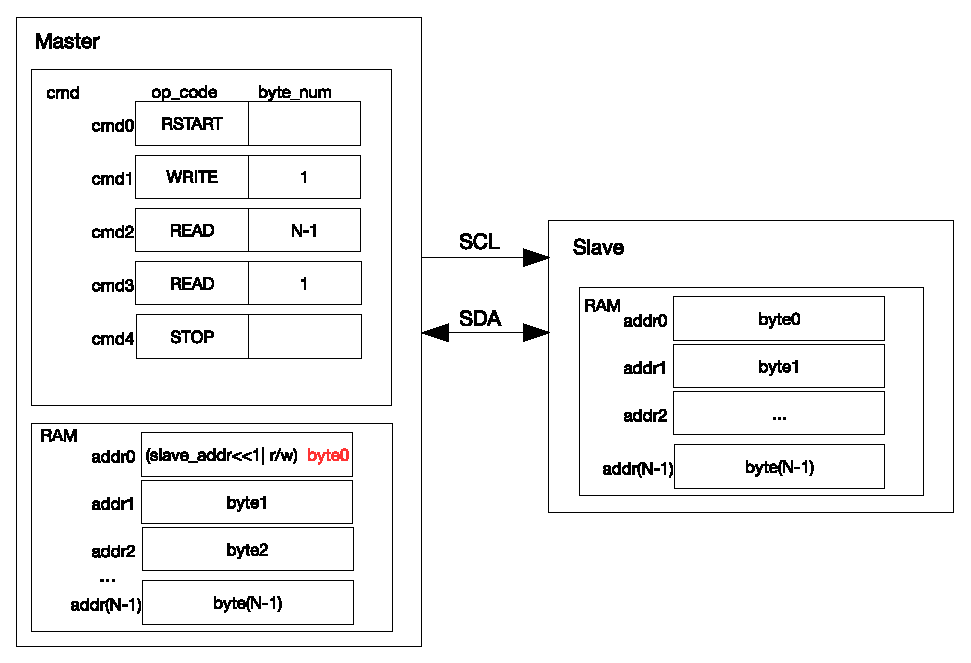
\includegraphics[width=0.8\textwidth]{\modulefiles/figures/I2C_MRS7}
    \caption{I2C 主机读 7 位寻址的从机}
    \label{fig:i2c-mrs7}
\end{figure}

图 \ref{fig:i2c-mrs7} I2C 主机从 7 位寻址 I2C 从机读取 N 个字节数据的寄存器或 RAM 的值。cmd1 为 WRITE 命令,I2C 主机会将 I2C 从机的地址发送出去。该命令发送的字节是7 位I2C 从机地址以及读写标志位。读写标志位为 1 表示读操作。I2C 从机在地址匹配成功之后即开始发送数据给 I2C 主机。I2C 主机根据 READ 命令中设置的 ack\_value ,在接收完一个字节的数据之后回复 ACK。

图 \ref{fig:i2c-mrs7} 中 READ 分成两次,I2C 主机对 cmd2 中 N-1 个数据均回复 ACK,对 cmd3 中的数据即传输的最后一个数据回复 NACK ,实际使用时可以根据需要进行配置。在存储接收的数据时,I2C 主机从RX RAM 的首地址开始存储,即为图中红色byte0存储的位置。

\subsubsection{配置示例}
\begin{enumerate}
\item 设置 \hyperref[fielddesc:I2CMSMODE]{I2C\_MS\_MODE}(主机)为1,\hyperref[fielddesc:I2CMSMODE]{I2C\_MS\_MODE}(从机)为0。
\item 推荐将 \hyperref[fielddesc:I2CSLAVESCLSTRETCHEN]{I2C\_SLAVE\_SCL\_STRETCH\_EN}(从机)置1,以便 I2C 从机在需要发送数据时可以先把SCL拉低来给软件向 I2C 从机的TX RAM中写数提供时间,否则 I2C 从机需要在主机开始传输前提前准备好数据。以下配置流程均按照\hyperref[fielddesc:I2CSLAVESCLSTRETCHEN]{I2C\_SLAVE\_SCL\_STRETCH\_EN}(从机)为1的情况进行。
\item 向 \hyperref[fielddesc:I2CCONFUPGATE]{I2C\_CONF\_UPGATE}(主机)和 \hyperref[fielddesc:I2CCONFUPGATE]{I2C\_CONF\_UPGATE}(从机)写1来同步寄存器。
\item 配置 I2C 主机的指令寄存器。
\clearpage
\begin{longtable}{ | p{4cm} | p{2cm} | p{2cm} | p{2cm} |p{2cm} | p{2cm} |}
\hline\rowcolor{lightgray}
指令寄存器& op\_code & ack\_value&ack\_exp&ack\_check\_en&byte\_num  \\ \hline
\hyperref[fielddesc:I2CCOMMAND0]{I2C\_COMMAND0}(主机)& RSTART& ---&---&---&---  \\ \hline
\hyperref[fielddesc:I2CCOMMAND1]{I2C\_COMMAND1}(主机)& WRITE& 0&0&1&1  \\ \hline
\hyperref[fielddesc:I2CCOMMAND2]{I2C\_COMMAND2}(主机)& READ& 0&0&1&N-1  \\ \hline
\hyperref[fielddesc:I2CCOMMAND3]{I2C\_COMMAND3}(主机)& READ& 1&0&1&1  \\ \hline
\hyperref[fielddesc:I2CCOMMAND4]{I2C\_COMMAND4}(主机)& STOP& ---&---&---&---  \\ \hline
\end{longtable}
\item 参考章节 \ref{subsubsec:i2c-txrx},向 I2C 主机的TX RAM写入从机地址。可选FIFO方式和直接访问方式。
\item 在\hyperref[regdesc:I2CSLAVEADDRREG]{I2C\_SLAVE\_ADDR\_REG}(从机)的\hyperref[fielddesc:I2CSLAVEADDR]{I2C\_SLAVE\_ADDR}(从机)设置 I2C 从机的地址。
\item 向 \hyperref[fielddesc:I2CCONFUPGATE]{I2C\_CONF\_UPGATE}(主机)和 \hyperref[fielddesc:I2CCONFUPGATE]{I2C\_CONF\_UPGATE}(从机)写1来同步寄存器。
\item 向 \hyperref[fielddesc:I2CTRANSSTART]{I2C\_TRANS\_START}(主机)写1开始主机的传输。
\item 参考章节 \ref{subsubsec:i2c-start},启动从机的传输。
\item I2C 从机比较 I2C 主机发送的从机地址和自己的\hyperref[fielddesc:I2CSLAVEADDR]{I2C\_SLAVE\_ADDR}(从机),当 I2C 主机 WRITE 命令中的 ack\_check\_en(主机) 配置为 1 时,I2C 主机会在发送完每个字节之后进行 ACK 检测。 若ack\_check\_en 配置为 0,则不会对ACK检测,会默认为匹配。
\begin{itemize}
\item 匹配:接收的 ACK 值与 WRITE 命令中的 ack\_exp(主机) 电平一致,传输继续。
\item 不匹配:接收的 ACK 值与 WRITE 命令中的 ack\_exp(主机) 电平不一致,I2C 主机产生 I2C\_NACK\_INT(主机) 中断,停止发送数据并且产生 STOP。
\end{itemize}

\item 等待\hyperref[int:i2c-slave-stretch]{I2C\_SLAVE\_STRETCH\_INT}(从机),读取 \hyperref[fielddesc:I2CSTRETCHCAUSE]{I2C\_STRETCH\_CAUSE} 的值为0,此时从机地址与SDA线上发送的地址相匹配,且从机要发送数据。
\item 参考章节 \ref{subsubsec:i2c-txrx},向 I2C 从机的TX RAM写入要发送的数据。可选FIFO方式和直接访问方式。
\item 将\hyperref[fielddesc:I2CSLAVESCLSTRETCHCLR]{I2C\_SLAVE\_SCL\_STRETCH\_CLR}(从机)置1,释放SCL总线。

\item I2C 从机发送数据,I2C 主机会根据当前READ指令对应的ack\_check\_en(主机) 配置的不同进行或不进行ACK检测。
\item 若 I2C 主机要读取的数超过32个,当发送数据全部发完,在 I2C 从机的TX RAM空时产生\hyperref[int:i2c-slave-stretch]{I2C\_SLAVE\_STRETCH\_INT}(从机)中断。此时 I2C 从机会将SCL拉低,软件在此期间可以继续向 I2C 从机的TX RAM填充数据,也可以从 I2C 主机的RX RAM读取数据。等完成操作后再将\hyperref[fielddesc:I2CSLAVESTRETCHINTCLR]{I2C\_SLAVE\_STRETCH\_INT\_CLR}(从机)置1清除中断,将 \hyperref[fielddesc:I2CSLAVESCLSTRETCHCLR]{I2C\_SLAVE\_SCL\_STRETCH\_CLR}(从机)置1释放SCL总线。

\item 当 I2C 主机接收最后一个数据时,将ack\_value(主机)设成1,I2C 从机接收到NACK中断,停止发送。

\item 当整个传输正常结束,I2C 主机执行STOP命令,并产生 I2C\_TRANS\_COMPLETE\_INT(主机) 中断。

\end{enumerate}

\subsection{I2C 主机读取从机,10 位寻址,单次命令序列}
\subsubsection{场景介绍}
\begin{figure}[H]
    \centering
    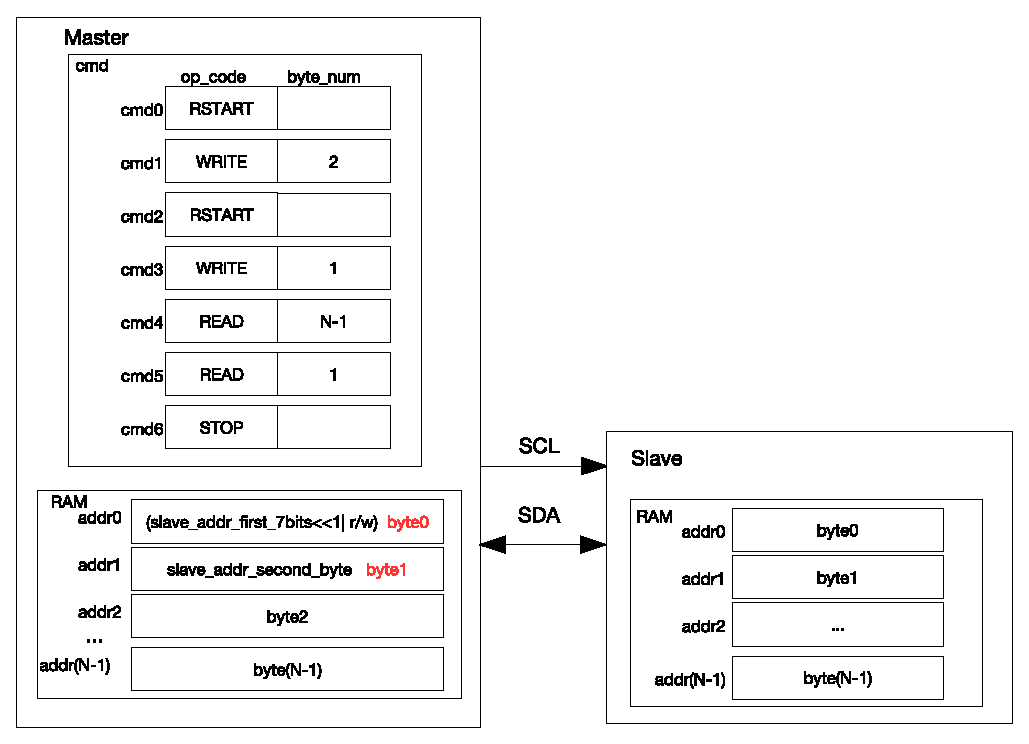
\includegraphics[width=0.8\textwidth]{\modulefiles/figures/I2C_MRS10}
    \caption{I2C 主机读 10 位寻址的从机}
    \label{fig:i2c-mrs10}
\end{figure}

图 \ref{fig:i2c-mrs10} 为 I2C 主机从 10 位 寻址的 I2C 从机中读取数据的寄存器或 RAM 的值。相比于 7 位寻址,I2C 主机的第一写命令的字节数为两个字节,相应TX RAM 中存储两个字节的 I2C 从机10 位地址,且第一个地址字节的R/W位为 W(主机)。之后再次发送RSTART,并重复发送第一个地址字节,R/W位为 R(从机)。之后主机从从机中读取数据。两个字节地址的配置方式与章节 \ref{sub:i2c-app-mws10} 的相同。

\subsubsection{配置示例}
\begin{enumerate}
\item 设置 \hyperref[fielddesc:I2CMSMODE]{I2C\_MS\_MODE}(主机)为1,\hyperref[fielddesc:I2CMSMODE]{I2C\_MS\_MODE}(从机)为0。
\item 推荐将 \hyperref[fielddesc:I2CSLAVESCLSTRETCHEN]{I2C\_SLAVE\_SCL\_STRETCH\_EN}(从机)置1,以便 I2C 从机在需要发送数据时可以先把SCL拉低来给软件向 I2C 从机的TX RAM中写数提供时间,否则 I2C 从机需要在主机开始传输前提前准备好数据。以下配置流程均按照\hyperref[fielddesc:I2CSLAVESCLSTRETCHEN]{I2C\_SLAVE\_SCL\_STRETCH\_EN}(从机)为1的情况进行。
\item 向 \hyperref[fielddesc:I2CCONFUPGATE]{I2C\_CONF\_UPGATE}(主机)和 \hyperref[fielddesc:I2CCONFUPGATE]{I2C\_CONF\_UPGATE}(从机)写1来同步寄存器。
\item 配置 I2C 主机的指令寄存器。
\begin{longtable}{ | p{4cm} | p{2cm} | p{2cm} | p{2cm} |p{2cm} | p{2cm} |}
\hline\rowcolor{lightgray}
指令寄存器& op\_code & ack\_value&ack\_exp&ack\_check\_en&byte\_num  \\ \hline
\hyperref[fielddesc:I2CCOMMAND0]{I2C\_COMMAND0}(主机)& RSTART& ---&---&---&---  \\ \hline
\hyperref[fielddesc:I2CCOMMAND1]{I2C\_COMMAND1}(主机)& WRITE& 0&0&1&2  \\ \hline
\hyperref[fielddesc:I2CCOMMAND2]{I2C\_COMMAND2}(主机)& RSTART& ---&---&---&---  \\ \hline
\hyperref[fielddesc:I2CCOMMAND3]{I2C\_COMMAND3}(主机)& WRITE& 0&0&1&1  \\ \hline
\hyperref[fielddesc:I2CCOMMAND4]{I2C\_COMMAND4}(主机)& READ& 0&0&1&N-1  \\ \hline
\hyperref[fielddesc:I2CCOMMAND5]{I2C\_COMMAND5}(主机)& READ& 1&0&1&1  \\ \hline
\hyperref[fielddesc:I2CCOMMAND6]{I2C\_COMMAND6}(主机)& STOP& ---&---&---&---  \\ \hline
\end{longtable}

\item 在\hyperref[regdesc:I2CSLAVEADDRREG]{I2C\_SLAVE\_ADDR\_REG}(从机)的\hyperref[fielddesc:I2CSLAVEADDR]{I2C\_SLAVE\_ADDR}(从机)设置 I2C 从机的10位从机地址,并将 \hyperref[fielddesc:I2CADDR10BITEN]{I2C\_ADDR\_10BIT\_EN}(从机)置1使能 10 位寻址模式。
\item 向 I2C 主机的TX RAM写入从机地址和要发送的数据,第一个地址字节是((0x{}78 | \hyperref[fielddesc:I2CSLAVEADDR]{I2C\_SLAVE\_ADDR}[9:8])<<1)|R/W,R/W位为 W(主机);第二个地址字节是\hyperref[fielddesc:I2CSLAVEADDR]{I2C\_SLAVE\_ADDR}[7:0]。第三个字节是重复的第一个地址字节加上R/W位,其中R/W位为 R(从机)。可选FIFO方式和直接访问方式。

\item 向 \hyperref[fielddesc:I2CCONFUPGATE]{I2C\_CONF\_UPGATE}(主机)和 \hyperref[fielddesc:I2CCONFUPGATE]{I2C\_CONF\_UPGATE}(从机)写1来同步寄存器。
\item 向 \hyperref[fielddesc:I2CTRANSSTART]{I2C\_TRANS\_START}(主机)写1开始主机的传输。
\item 参考章节 \ref{subsubsec:i2c-start},启动从机的传输。
\item I2C 从机比较 I2C 主机发送的从机地址和自己的\hyperref[fielddesc:I2CSLAVEADDR]{I2C\_SLAVE\_ADDR}(从机),当 I2C 主机 WRITE 命令中的 ack\_check\_en(主机) 配置为 1 时,I2C 主机会在发送完每个字节之后进行 ACK 检测。 若ack\_check\_en 配置为 0,则不会对ACK检测,会默认为匹配。
\begin{itemize}
\item 匹配:接收的 ACK 值与 WRITE 命令中的 ack\_exp(主机) 电平一致,传输继续。
\item 不匹配:接收的 ACK 值与 WRITE 命令中的 ack\_exp(主机) 电平不一致,I2C 主机产生 I2C\_NACK\_INT(主机) 中断,停止发送数据并且产生 STOP。
\end{itemize}

\item I2C 主机 发送RSTART命令,并发送TX RAM里的第三个字节,即为重复的地址字节和R 位。
\item I2C 从机重复执行步骤10,若地址匹配,继续后面的步骤。

\item 等待\hyperref[int:i2c-slave-stretch]{I2C\_SLAVE\_STRETCH\_INT}(从机),读取 \hyperref[fielddesc:I2CSTRETCHCAUSE]{I2C\_STRETCH\_CAUSE} 的值为0,此时从机地址与SDA线上发送的地址相匹配,且从机要发送数据。
\item 参考章节 \ref{subsubsec:i2c-txrx},向 I2C 从机的TX RAM写入要发送的数据。可选FIFO方式和直接访问方式。
\item 将\hyperref[fielddesc:I2CSLAVESCLSTRETCHCLR]{I2C\_SLAVE\_SCL\_STRETCH\_CLR}(从机)置1,释放SCL总线。


\item I2C 从机发送数据,I2C 主机会根据当前READ指令对应的ack\_check\_en(主机) 配置的不同进行或不进行ACK检测。
\item 若 I2C 主机要读取的数超过32个字节,当发送数据全部发完,在 I2C 从机的TX RAM空时产生 \\\hyperref[int:i2c-slave-stretch]{I2C\_SLAVE\_STRETCH\_INT}(从机)中断。此时 I2C 从机会将SCL拉低,软件在此期间可以继续向 I2C 从机的TX RAM填充数据,也可以从 I2C 主机的RX RAM读取数据。等完成操作后再将 \hyperref[fielddesc:I2CSLAVESTRETCHINTCLR]{I2C\_SLAVE\_STRETCH\_INT\_CLR}(从机)置1 清除中断,将\hyperref[fielddesc:I2CSLAVESCLSTRETCHCLR]{I2C\_SLAVE\_SCL\_STRETCH\_CLR}(从机)置1 释放SCL总线。

\item 当 I2C 主机接收最后一个数据时,将ack\_value(主机)设成1,I2C 从机接收到NACK中断,停止发送。

\item 当整个传输正常结束,I2C 主机执行STOP命令,并产生 I2C\_TRANS\_COMPLETE\_INT(主机) 中断。
\end{enumerate}

\subsection{I2C 主机读取从机,7 位双寻址,单次命令序列}
\subsubsection{场景介绍}
\begin{figure}[H]
    \centering
    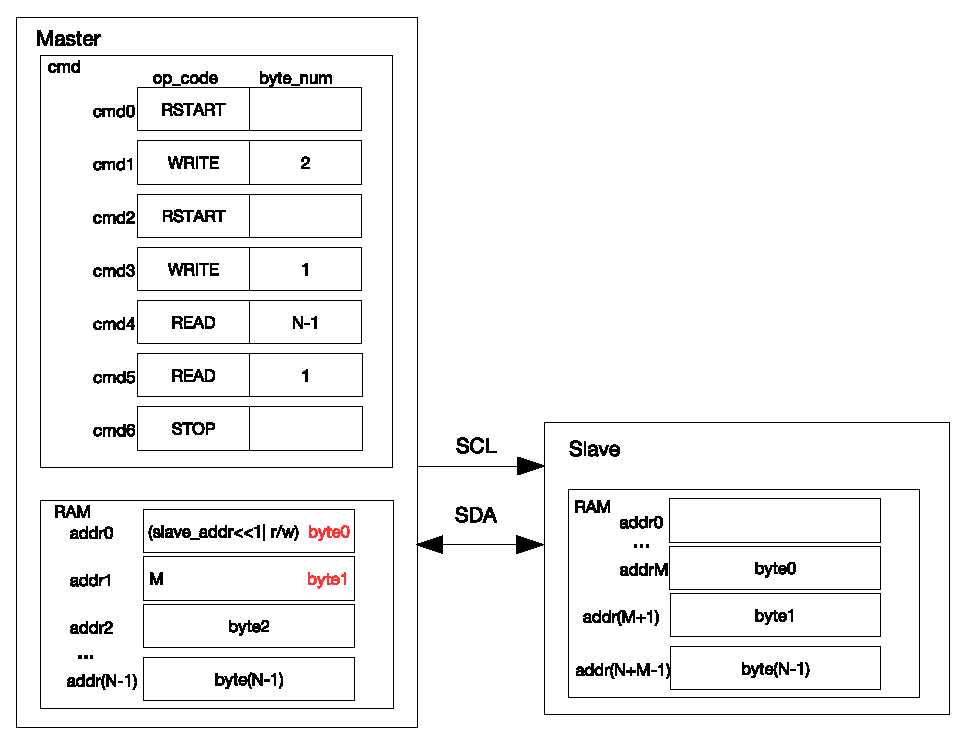
\includegraphics[width=0.8\textwidth]{\modulefiles/figures/I2C_MRS7_M}
    \caption{I2C 主机从 7 位寻址 从机的 M 地址读取 N 个数据}
    \label{fig:i2c-mrs7-m}
\end{figure}

图 \ref{fig:i2c-mrs7-m} 为 I2C 主机从 I2C 从机中指定地址读取数据的寄存器或 RAM 的值。主机在传输开始发送2个地址字节,第一个地址字节是从机的 7 位地址加R/W位,R/W位为 W(主机);第二个地址字节是从机的内存地址M。之后再次发送RSTART,并重复发送第一个地址字节,R/W位变为 R(从机)。之后主机从从机的AddrM地址开始读取数据。

\subsubsection{配置示例}
\begin{enumerate}
\item 设置 \hyperref[fielddesc:I2CMSMODE]{I2C\_MS\_MODE}(主机)为1,\hyperref[fielddesc:I2CMSMODE]{I2C\_MS\_MODE}(从机)为0。
\item 推荐将 \hyperref[fielddesc:I2CSLAVESCLSTRETCHEN]{I2C\_SLAVE\_SCL\_STRETCH\_EN}(从机)置1,以便 I2C 从机在需要发送数据时可以先把SCL拉低来给软件向 I2C 从机的TX RAM中写数提供时间,否则 I2C 从机需要在主机开始传输前提前准备好数据。以下配置流程均按照\hyperref[fielddesc:I2CSLAVESCLSTRETCHEN]{I2C\_SLAVE\_SCL\_STRETCH\_EN}(从机)为1的情况进行。
\item 设置\hyperref[fielddesc:I2CFIFOADDRCFGEN]{I2C\_FIFO\_ADDR\_CFG\_EN}(从机)为1来使能双寻址模式。
\item 向 \hyperref[fielddesc:I2CCONFUPGATE]{I2C\_CONF\_UPGATE}(主机)和 \hyperref[fielddesc:I2CCONFUPGATE]{I2C\_CONF\_UPGATE}(从机)写1来同步寄存器。
\item 配置 I2C 主机的指令寄存器。
\begin{longtable}{ | p{4cm} | p{2cm} | p{2cm} | p{2cm} |p{2cm} | p{2cm} |}
\hline\rowcolor{lightgray}
指令寄存器& op\_code & ack\_value&ack\_exp&ack\_check\_en&byte\_num  \\ \hline
\hyperref[fielddesc:I2CCOMMAND0]{I2C\_COMMAND0}(主机)& RSTART& ---&---&---&---  \\ \hline
\hyperref[fielddesc:I2CCOMMAND1]{I2C\_COMMAND1}(主机)& WRITE& 0&0&1&2  \\ \hline
\hyperref[fielddesc:I2CCOMMAND2]{I2C\_COMMAND2}(主机)& RSTART& ---&---&---&---  \\ \hline
\hyperref[fielddesc:I2CCOMMAND3]{I2C\_COMMAND3}(主机)& WRITE& 0&0&1&1  \\ \hline
\hyperref[fielddesc:I2CCOMMAND4]{I2C\_COMMAND4}(主机)& READ& 0&0&1&N-1  \\ \hline
\hyperref[fielddesc:I2CCOMMAND5]{I2C\_COMMAND5}(主机)& READ& 1&0&1&1  \\ \hline
\hyperref[fielddesc:I2CCOMMAND6]{I2C\_COMMAND6}(主机)& STOP& ---&---&---&---  \\ \hline
\end{longtable}

\item 在\hyperref[regdesc:I2CSLAVEADDRREG]{I2C\_SLAVE\_ADDR\_REG}(从机)的 \hyperref[fielddesc:I2CSLAVEADDR]{I2C\_SLAVE\_ADDR}(从机)设置 I2C 从机的7位地址,\hyperref[fielddesc:I2CADDR10BITEN]{I2C\_ADDR\_10BIT\_EN}(从机)置0使能 7 位寻址模式。
\item 参考章节 \ref{subsubsec:i2c-txrx},向 I2C 主机的TX RAM写入从机地址和要发送的数据,第一个地址字节是 \\( \hyperref[fielddesc:I2CSLAVEADDR]{I2C\_SLAVE\_ADDR}[6:0])<<1)|R/W,R/W位为 W(主机);第二个地址字节是 I2C 从机的内存地址M。第三个字节是重复的第一个地址字节加上R/W位,其中R/W位为 R(从机)。可选FIFO方式和直接访问方式。

\item 向 \hyperref[fielddesc:I2CCONFUPGATE]{I2C\_CONF\_UPGATE}(主机)和 \hyperref[fielddesc:I2CCONFUPGATE]{I2C\_CONF\_UPGATE}(从机)写1来同步寄存器。
\item 向 \hyperref[fielddesc:I2CTRANSSTART]{I2C\_TRANS\_START}(主机)写1开始主机的传输。
\item 参考章节 \ref{subsubsec:i2c-start},启动 I2C 从机的传输。


\item I2C 从机比较 I2C 主机发送的从机地址和自己的\hyperref[fielddesc:I2CSLAVEADDR]{I2C\_SLAVE\_ADDR}(从机),当 I2C 主机 WRITE 命令中的 ack\_check\_en(主机) 配置为 1 时,I2C 主机会在发送完每个字节之后进行 ACK 检测。 若ack\_check\_en 配置为 0,则不会对ACK检测,会默认为匹配。
\begin{itemize}
\item 匹配:接收的 ACK 值与 WRITE 命令中的 ack\_exp(主机) 电平一致,传输继续。
\item 不匹配:接收的 ACK 值与 WRITE 命令中的 ack\_exp(主机) 电平不一致,I2C 主机产生 I2C\_NACK\_INT(主机) 中断,停止发送数据并且产生 STOP。
\end{itemize}
\item I2C 从机接收到 I2C 主机发送的内存地址,完成TX RAM的地址偏移。
\item I2C 主机 发送RSTART命令,并发送TX RAM里的第三个字节,即为重复的地址字节和R 位。
\item I2C 从机重复执行步骤11,若地址匹配,继续后面的步骤。

\item 等待\hyperref[int:i2c-slave-stretch]{I2C\_SLAVE\_STRETCH\_INT}(从机),读取 \hyperref[fielddesc:I2CSTRETCHCAUSE]{I2C\_STRETCH\_CAUSE} 的值为0,此时从机地址与SDA线上发送的地址相匹配,且从机要发送数据。

\item 参考章节 \ref{subsubsec:i2c-txrx},向 I2C 从机的TX RAM写入要发送的数据。可选FIFO方式和直接访问方式。
\item 将\hyperref[fielddesc:I2CSLAVESCLSTRETCHCLR]{I2C\_SLAVE\_SCL\_STRETCH\_CLR}(从机)置1,释放SCL总线。


\item I2C 从机发送数据,I2C 主机会根据当前READ指令对应的ack\_check\_en(主机) 配置的不同进行或不进行ACK检测。
\item 若 I2C 主机要读取的数超过32个,当发送数据全部发完,在 I2C 从机的TX RAM空时产生\hyperref[int:i2c-slave-stretch]{I2C\_SLAVE\_STRETCH\_INT}(从机)中断。此时 I2C 从机会将SCL拉低,软件在此期间可以继续向 I2C 从机的TX RAM填充数据,也可以从 I2C 主机的RX RAM读取数据。等完成操作后再将\hyperref[fielddesc:I2CSLAVESTRETCHINTCLR]{I2C\_SLAVE\_STRETCH\_INT\_CLR}(从机)置1,清除中断;\hyperref[fielddesc:I2CSLAVESCLSTRETCHCLR]{I2C\_SLAVE\_SCL\_STRETCH\_CLR}(从机)置1,释放SCL总线。

\item 当 I2C 主机接收最后一个数据时,将ack\_value(主机)设成1,I2C 从机接收到NACK中断,停止发送。

\item 当整个传输正常结束,I2C 主机执行STOP命令,并产生 I2C\_TRANS\_COMPLETE\_INT(主机) 中断。
\end{enumerate}


\subsection{I2C 主机读取从机,7 位寻址,多次命令序列}
\subsubsection{场景介绍}
\begin{figure}[H]
    \centering
    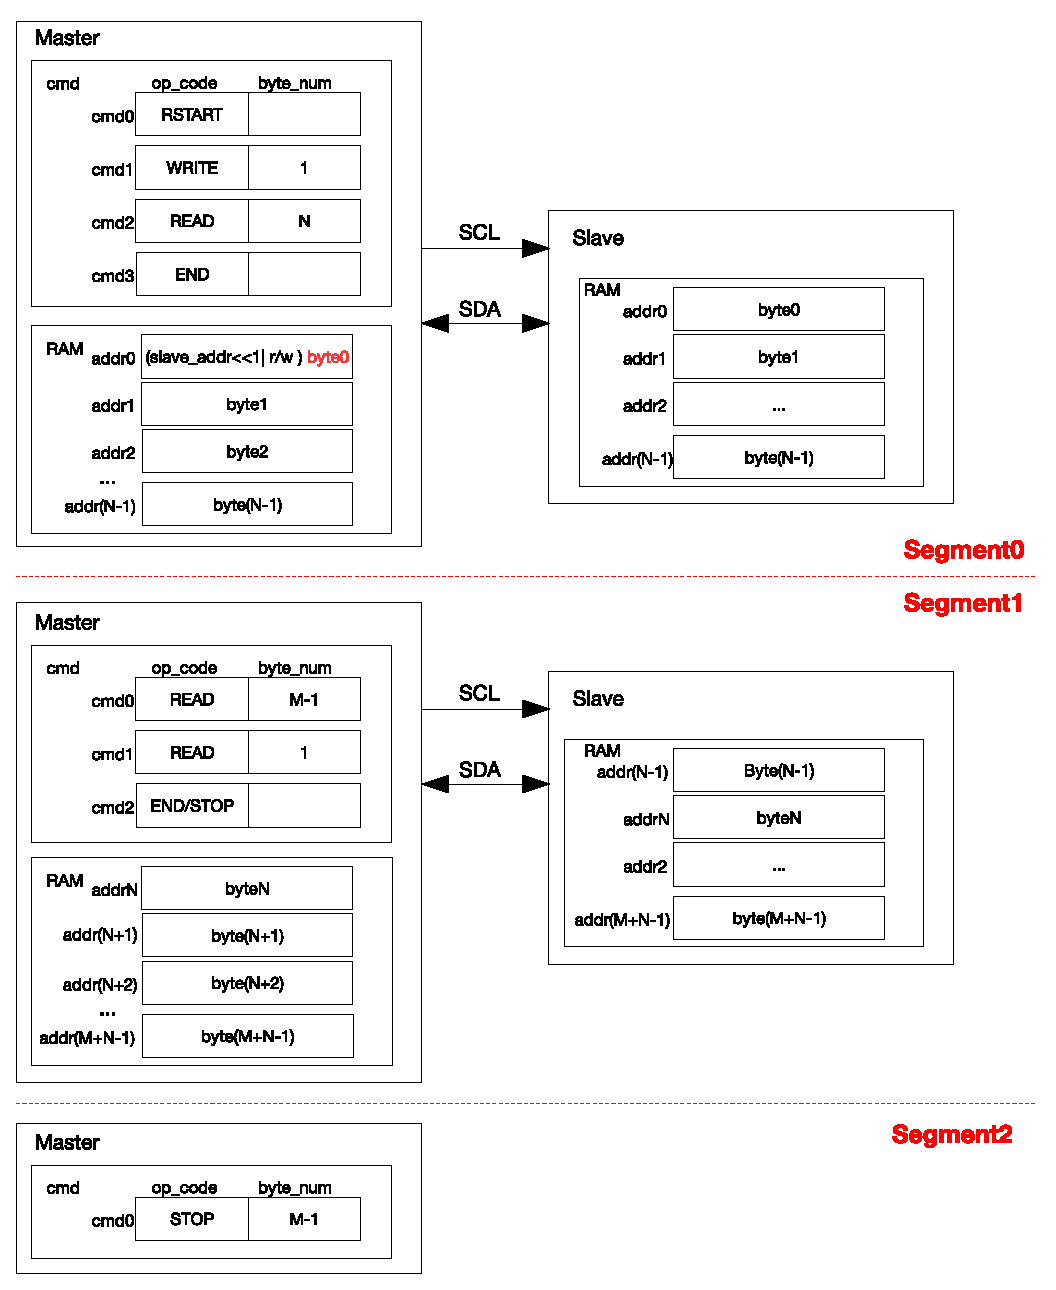
\includegraphics[width=0.8\textwidth]{\modulefiles/figures/I2C_MRS_END}
    \caption{I2C 主机分段读 7 位寻址的从机}
    \label{fig:i2c-mrs7-multiple}
\end{figure}

图 \ref{fig:i2c-mrs7-multiple} 为 I2C 主机通过 END 命令分三段或者分两段,从 I2C 从机读取 N+M 个数据的流程图。
\begin{enumerate}
    \item 第一段流程和 \ref{fig:i2c-mrs7}类似,只是最后一个命令变为END。
    \item 接着在 从机的TX RAM 中准备好数据,置位 \hyperref[fielddesc:I2CTRANSSTART]{I2C\_TRANS\_START},当执行到 END 命令时,I2C 主机可以更新命令寄存器和RAM的内容,如第二段所示,并且清零其对应的 I2C\_END\_DETECT\_INT 中断。当第二段中 cmd2 为 STOP 时,即两段读 I2C从机,置位 \hyperref[fielddesc:I2CTRANSSTART]{I2C\_TRANS\_START},I2C 主机继续传输数据,最后发送 STOP 位来停止传输。
    \item 当第二段中 cmd2 为 END 时,在 I2C 主机完成第二次数据传输,并检测到 I2C 主机的 I2C\_END\_DETECT\_INT 中断后,配置 cmd 如第三段所示。置位 \hyperref[fielddesc:I2CTRANSSTART]{I2C\_TRANS\_START},I2C 主机发送 STOP 位停止传输。
\end{enumerate}

\subsubsection{配置示例}
\begin{enumerate}
\item 设置 \hyperref[fielddesc:I2CMSMODE]{I2C\_MS\_MODE}(主机)为1,\hyperref[fielddesc:I2CMSMODE]{I2C\_MS\_MODE}(从机)为0。
\item 推荐将 \hyperref[fielddesc:I2CSLAVESCLSTRETCHEN]{I2C\_SLAVE\_SCL\_STRETCH\_EN}(从机)置1,以便 I2C 从机在需要发送数据时可以先把SCL拉低来给软件向 I2C 从机的TX RAM中写数提供时间,否则 I2C 从机需要在主机开始传输前提前准备好数据。以下配置流程均按照\hyperref[fielddesc:I2CSLAVESCLSTRETCHEN]{I2C\_SLAVE\_SCL\_STRETCH\_EN}(从机)为1的情况进行。
\item 向 \hyperref[fielddesc:I2CCONFUPGATE]{I2C\_CONF\_UPGATE}(主机)和 \hyperref[fielddesc:I2CCONFUPGATE]{I2C\_CONF\_UPGATE}(从机)写1来同步寄存器。
\item 配置 I2C 主机的指令寄存器。
\begin{longtable}{ | p{4cm} | p{2cm} | p{2cm} | p{2cm} |p{2cm} | p{2cm} |}
\hline\rowcolor{lightgray}
指令寄存器& op\_code & ack\_value&ack\_exp&ack\_check\_en&byte\_num  \\ \hline
\hyperref[fielddesc:I2CCOMMAND0]{I2C\_COMMAND0}(主机)& RSTART& ---&---&---&---  \\ \hline
\hyperref[fielddesc:I2CCOMMAND1]{I2C\_COMMAND1}(主机)& WRITE& 0&0&1&1  \\ \hline
\hyperref[fielddesc:I2CCOMMAND2]{I2C\_COMMAND2}(主机)& READ& 0&0&1&N  \\ \hline
\hyperref[fielddesc:I2CCOMMAND3]{I2C\_COMMAND3}(主机)& END& ---&---&---&---  \\ \hline
\end{longtable}
\item 向 I2C 主机的TX RAM写入从机地址,可选FIFO方式和直接访问方式。
\item 在\hyperref[regdesc:I2CSLAVEADDRREG]{I2C\_SLAVE\_ADDR\_REG}(从机)的\hyperref[fielddesc:I2CSLAVEADDR]{I2C\_SLAVE\_ADDR}(从机)设置 I2C 从机的地址。
\item 向 \hyperref[fielddesc:I2CCONFUPGATE]{I2C\_CONF\_UPGATE}(主机)和 \hyperref[fielddesc:I2CCONFUPGATE]{I2C\_CONF\_UPGATE}(从机)写1来同步寄存器。
\item 向 \hyperref[fielddesc:I2CTRANSSTART]{I2C\_TRANS\_START}(主机)写1开始主机的传输。
\item 参考章节 \ref{subsubsec:i2c-start},启动从机的传输。
\item I2C 从机比较 I2C 主机发送的从机地址和自己的\hyperref[fielddesc:I2CSLAVEADDR]{I2C\_SLAVE\_ADDR}(从机),当 I2C 主机 WRITE 命令中的 ack\_check\_en(主机) 配置为 1 时,I2C 主机会在发送完每个字节之后进行 ACK 检测。 若ack\_check\_en 配置为 0,则不会对ACK检测,会默认为匹配。
\begin{itemize}
\item 匹配:接收的 ACK 值与 WRITE 命令中的 ack\_exp(主机) 电平一致,传输继续。
\item 不匹配:接收的 ACK 值与 WRITE 命令中的 ack\_exp(主机) 电平不一致,I2C 主机产生 I2C\_NACK\_INT(主机) 中断,停止发送数据并且产生 STOP。
\end{itemize}

\item 等待\hyperref[int:i2c-slave-stretch]{I2C\_SLAVE\_STRETCH\_INT}(从机),读取 \hyperref[fielddesc:I2CSTRETCHCAUSE]{I2C\_STRETCH\_CAUSE} 的值为0,此时从机地址与SDA线上发送的地址相匹配,且从机要发送数据。

\item 参考章节 \ref{subsubsec:i2c-txrx},向 I2C 从机的TX RAM写入要发送的数据。可选FIFO方式和直接访问方式。
\item 将\hyperref[fielddesc:I2CSLAVESCLSTRETCHCLR]{I2C\_SLAVE\_SCL\_STRETCH\_CLR}(从机)置1,释放SCL总线。

\item I2C 从机发送数据,I2C 主机会根据当前READ指令对应的ack\_check\_en(主机) 配置的不同进行或不进行ACK检测。
\item 若 I2C 主机一个READ指令要读取的数N或M超过32个字节,当 I2C 从机的TX RAM中发送数据全部发完,为空时产生\hyperref[int:i2c-slave-stretch]{I2C\_SLAVE\_STRETCH\_INT}(从机)中断。此时 I2C 从机会将SCL拉低,软件在此期间可以继续向 I2C 从机的TX RAM填充数据,也可以从 I2C 主机的RX RAM读取数据。等完成操作后再将\hyperref[fielddesc:I2CSLAVESTRETCHINTCLR]{I2C\_SLAVE\_STRETCH\_INT\_CLR}(从机)置1清除中断,将 \hyperref[fielddesc:I2CSLAVESCLSTRETCHCLR]{I2C\_SLAVE\_SCL\_STRETCH\_CLR}(从机)置1释放SCL总线。

\item 等到一次READ指令完成,I2C 主机执行END指令,I2C\_END\_DETECT\_INT(主机)中断产生后,设置 \hyperref[fielddesc:I2CENDDETECTINTCLR]{I2C\_END\_DETECT\_INT\_CLR}(主机)为1来清除中断。

\clearpage
\item 更新 I2C 主机的指令寄存器,有两种设置方式:

\begin{longtable}{ | p{4cm} | p{2cm} | p{2cm} | p{2cm} |p{2cm} | p{2cm} |}
\hline\rowcolor{lightgray}
指令寄存器& op\_code & ack\_value&ack\_exp&ack\_check\_en&byte\_num  \\ \hline
\hyperref[fielddesc:I2CCOMMAND0]{I2C\_COMMAND0}(主机)& READ& ack\_value&ack\_exp&1&M  \\ \hline
\hyperref[fielddesc:I2CCOMMAND1]{I2C\_COMMAND1}(主机)& END& ---&---&---&---  \\ \hline
\end{longtable}

或者

\begin{longtable}{ | p{4cm} | p{2cm} | p{2cm} | p{2cm} |p{2cm} | p{2cm} |}
\hline\rowcolor{lightgray}
指令寄存器& op\_code & ack\_value&ack\_exp&ack\_check\_en&byte\_num  \\ \hline
\hyperref[fielddesc:I2CCOMMAND0]{I2C\_COMMAND0}(主机)& READ& 0&0&1&M-1  \\ \hline
\hyperref[fielddesc:I2CCOMMAND0]{I2C\_COMMAND0}(主机)& READ& 1&0&1&1  \\ \hline
\hyperref[fielddesc:I2CCOMMAND1]{I2C\_COMMAND1}(主机)& STOP& ---&---&---&---  \\ \hline
\end{longtable}

\item 向 I2C 从机的TX RAM写入M个字节要发送的数据,若M大于32,重复步骤12,可以用FIFO方式或直接访问方式。
\item 向 \hyperref[fielddesc:I2CTRANSSTART]{I2C\_TRANS\_START}(主机)位写1开始传输,并重复步骤14的流程。
\item 若最后一个指令为STOP,则当 I2C 主机接收最后一个数据时,将ack\_value(主机)设成1,I2C 从机接收到NACK中断,停止发送。 I2C 主机执行STOP命令结束传输,并产生I2C\_TRANS\_COMPLETE\_INT(主机)中断。
\item 若最后一个指令为为END,则重复步骤16,并在完成后继续下面的步骤。
\item 更新 I2C 主机的指令寄存器。
\begin{longtable}{ | p{4cm} | p{2cm} | p{2cm} | p{2cm} |p{2cm} | p{2cm} |}
\hline\rowcolor{lightgray}
指令寄存器& op\_code & ack\_value&ack\_exp&ack\_check\_en&byte\_num  \\ \hline
\hyperref[fielddesc:I2CCOMMAND1]{I2C\_COMMAND1}(主机)& STOP& ---&---&---&---  \\ \hline
\end{longtable}
\item 向 \hyperref[fielddesc:I2CTRANSSTART]{I2C\_TRANS\_START}(主机)位写1开始传输。
\item I2C 主机执行STOP命令结束传输,并产生I2C\_TRANS\_COMPLETE\_INT(主机)中断。

\end{enumerate}

\section{中断}\label{sub:i2c-int}
\begin{itemize}
\item \label{int:i2c-slave-stretch}I2C\_SLAVE\_STRETCH\_INT:从机模式下,当出现可触发时钟拉伸的时,产生此中断。
\item \label{int:i2c-start}I2C\_DET\_START\_INT:主机或从机检测到I2C START位时,触发此中断。
\item \label{int:i2c-scl-main-fsm}I2C\_SCL\_MAIN\_ST\_TO\_INT:当I2C主状态机SCL\_MAIN\_FSM保持某个状态超过 \hyperref[fielddesc:I2CSCLMAINSTTOI2C]{I2C\_SCL\_MAIN\_ST\_TO\_I2C}[23:0]个模块时钟周期时,触发此中断。
\item \label{int:i2c-scl-fsm}I2C\_SCL\_ST\_TO\_INT:当I2C状态机SCL\_FSM保持某个状态超过 \hyperref[fielddesc:I2CSCLSTTOI2C]{I2C\_SCL\_ST\_TO\_I2C}[23:0]个模块时钟周期时,触发此中断。
\item \label{int:i2c-rxfifo-udf}I2C\_RXFIFO\_UDF\_INT: 当 I2C 通过 APB 总线读取 RX FIFO,但 RX FIFO 为空时,触发该中断。
\item \label{int:i2c-txfifo-ovf}I2C\_TXFIFO\_OVF\_INT: 当 I2C 通过 APB 总线写 TX FIFO,但 TX FIFO 为满时,触发该中断。
\item \label{int:i2c-nack}I2C\_NACK\_INT: 当 I2C 配置为 主机时,接收到的 ACK 与命令中期望的 ACK 值不一致时,即触发该中断;当 I2C 配置为 从机时,接收到的 ACK 值为 1 时即触发该中断。
\item \label{int:i2c-trans-start}I2C\_TRANS\_START\_INT: 当 I2C 发送一个 START 位时,即触发该中断。
\item \label{int:i2c-time-out}I2C\_TIME\_OUT\_INT: 在传输过程中,当 I2C SCL 保持为高或为低电平的时间超过 2$^{\hyperref[fielddesc:I2CTIMEOUTVALUE]{I2C\_TIME\_OUT\_VALUE}}$ 个模块时钟后,即触发该中断。
\item \label{int:i2c-trans-complete}I2C\_TRANS\_COMPLETE\_INT: 当 I2C 检测到 STOP 位时,即触发该中断。
\item \label{int:i2c-mst-txfifo-udf}I2C\_MST\_TXFIFO\_UDF\_INT: 当 I2C 主机的TX FIFO 下溢时,触发此中断。
\item \label{int:i2c-arbitration-lost}I2C\_ARBITRATION\_LOST\_INT: 当 I2C 主机的 SCL 为高电平,SDA 输出值与输入值不相等时,即触发该中断。
\item \label{int:i2c-byte-trans-done}I2C\_BYTE\_TRANS\_DONE\_INT: 当 I2C 发送或接收一个字节,即触发该中断。
\item \label{int:i2c-end}I2C\_END\_DETECT\_INT:当I2C 主机命令的op\_code为END,且检测到 I2C END 状态时,触发此中断。
\item \label{int:i2c-rxfifo-ovf}I2C\_RXFIFO\_OVF\_INT:当I2C RX FIFO上溢时,触发此中断。
\item \label{int:i2c-txfifo-wm}I2C\_TXFIFO\_WM\_INT:I2C TX FIFO 水标中断。 当\hyperref[fielddesc:I2CFIFOPRTEN]{I2C\_FIFO\_PRT\_EN} 为1,且 TX FIFO 指针小于

\hyperref[fielddesc:I2CTXFIFOWMTHRHD]{I2C\_TXFIFO\_WM\_THRHD}[4:0]时,触发此中断。
\item \label{int:i2c-rxfifo-wm}I2C\_RXFIFO\_WM\_INT:I2C RX FIFO 水标中断。 当\hyperref[fielddesc:I2CFIFOPRTEN]{I2C\_FIFO\_PRT\_EN} 为1,且 RX FIFO 指针大于

\hyperref[fielddesc:I2CRXFIFOWMTHRHD]{I2C\_RXFIFO\_WM\_THRHD}[4:0]时,触发此中断。
\end{itemize}


%%%%%%%%%%%%%%%%%%%%%%%%
%%% Register Summary %%%
%%%%%%%%%%%%%%%%%%%%%%%%

\clearpage
\section{寄存器列表}
\label{sec:i2c-reg-summ}
\hypertarget{i2c-reg-summ}{}

本小节的所有地址均为相对于 \textcolor{red}{I2C 控制器} 基地址的地址偏移量(相对地址),具体基地址请见章节 \ref{mod:sysmem} \textit{\nameref{mod:sysmem}} 中的表 \ref{tab:sysmem-base-address}。

请查看章节 \hyperref[glossary-access-types]{\textit{寄存器的访问类型}},了解“访问”列缩写的含义。

\subfile{\modulefiles/01-I2C-reg-summ__CN}


%%%%%%%%%%%%%%%%%
%%% Registers %%%
%%%%%%%%%%%%%%%%%

\clearpage
\section{寄存器}

本小节的所有地址均为相对于 \textcolor{red}{I2C 控制器} 基地址的地址偏移量(相对地址),具体基地址请见章节 \ref{mod:sysmem} \textit{\nameref{mod:sysmem}} 中的表 \ref{tab:sysmem-base-address}。

\subfile{\modulefiles/01-I2C-reg__CN}


\end{document}
